%%%%%%%%%%%%%%%%%%%%%%%%%%%%%%%%%%%%%%
% This is the name of the style file.
%%%%%%%%%%%%%%%%%%%%%%%%%%%%%%%%%%%%%%
%
% phd  -> for a PhD dissertation
% ms   -> for an MS thesis
% If both phd and ms are used then phd will overide.  If none are used,
% then ms will be active by default.
%
% cpyr -> generate a copyright page
% lof  -> generate List of Figures
% lot  -> generate List of Tables
\documentclass[ms,cpyr,lof,lot]{uathesis}
%
%%%%%%%%%%%%%%%%%%%%%%%%%%%%%%%%
% List of any packages you use.
%%%%%%%%%%%%%%%%%%%%%%%%%%%%%%%%
%

\usepackage[nounderscore]{syntax}
\usepackage{listings}
\usepackage{algorithm, algpseudocode}
\usepackage[linewidth=1pt]{mdframed}
\usepackage{setspace}
\usepackage{amsmath}
\usepackage{amssymb}
\usepackage{epsfig}
\usepackage{graphicx}
\usepackage{changebar}
\usepackage{url}
\usepackage{environ}

\lstset{basicstyle=\ttfamily\singlespacing\small,
	    emph={layout, int, uint, decoder, extract, as, var, else, if, requires, exact_table, event, output, decode, goto, advance, drop, flood, set, write, clear, raise, insert, into, remove, from, match, case, while, miss, break, continue, Port, return, def},
	    emph=[2]{ start, in\_port, in\_phys\_port, egress, reflow, controller, all, timeout },
	    emph=[3]{ Error },
	    emphstyle={\color{blue}\textbf},
	    emphstyle=[2]{\color{green}\textbf},
	    emphstyle=[3]{\color{red}},
	    frame=single,
	    tabsize=2}

\graphicspath{ {./images/} }

\setlength{\medmuskip}{0mu}

\newlength{\currentparskip}
\newenvironment{minip}
  {\noindent\setlength{\currentparskip}{\parskip}% save the value
   \begin{minipage}{\textwidth}% open the minipage
   \singlespace
   \setlength{\parskip}{\currentparskip}% restore the value
  }
  {\end{minipage}\vspace{\baselineskip}}


%\noindent\begin{minipage}{\linewidth}
%\begin{grammar}
%\singlespace
%
%
%\end{grammar}
%\end{minipage}


%
%%%%%%%%%%%%%%%%%%%%%%%%%%%%%%%%%%
% List of definitions you define.
%%%%%%%%%%%%%%%%%%%%%%%%%%%%%%%%%%
%
\def\ds{\displaystyle}
\def\E{\epsilon}
\def\la{\langle}
\def\ra{\rangle}
\def\mn{\text{-}}
\newcommand\grdd[3]{$\la #1 \mn #2 \mn #3 \ra$}
\newcommand\grd[2]{$\la #1 \mn #2 \ra$}
\newcommand\gr[1]{$\la #1 \ra$}

%

\title{Steve - A Programming Language for Packet Processing}
\author{Hoang Nguyen}
\conferraldate{May}{2016}

%The following commands specify the names and titles of people that
%will appear on the signature page.
%
%These four will always be needed.
\advisor{Andrew Sutton}
\chair{Timothy O'Neil}
\collegedean{John Green}
\gradschdean{Chand Midha}
%
%For a PhD dissertation, specify a coadvisor and three committee
%members, or four committee members only.  For an MS thesis use either
%one coadvisor or one faculty reader, not both.
%
%Typical commands for a PhD dissertation (uncomment only 4).
%\coadvisor{Name of Coadvisor}
\committee{Name of 1st Comm Member}
\committee{Name of 2nd Comm Member}
\committee{Name of 3rd Comm Member}
\committee{Name of 4th Comm Member}
%
%Typical commands for an MS thesis (uncomment only 1).
%\coadvisor{Andrew Sutton}
\facreader{NAME 1}
\facreader{NAME 2}

\begin{document}
\maketitle
\chapter{INTRODUCTION} \label{ch:intro}

The wave equation can be used to describe many physical phenomena.
Challenging topics in meteorology, acoustics, electro-magnetics, and
others involve solving the time-dependent wave equation.  Many of
these problems are described in an unbounded domain (i.e. there is no
boundary to reflect the outward traveling waves).  When an exact,
theoretical solution is unavailable, the lack of a boundary
prescription of accurate radiation conditions creates a problem for
numerical solutions.  The difficulty lies in is finding a way to do
calculations on an infinite domain using a computer with finite memory
in a finite amount of time and within a finite region.

\chapter{THE TWO DIMENSIONAL WAVE EQUATION} \label{2DWaveEquation}

Here is an example of a 'section' and a few equations.

\section{Recurrence Relation}

A series solution for the two-dimensional wave equation
\begin{equation}
\frac{1}{c^{2}}\frac{\partial^{2}u}{\partial t^{2}} = \frac{\partial^{2}u}{\partial r^{2}} + %
        \frac{1}{r}\frac{\partial u}{\partial r} + \frac{1}{r^{2}}\frac{\partial^{2}u}%
        {\partial\theta^{2}}                                                                 \label{waveEq}
\end{equation}
for outgoing waves is
\begin{equation}
u = \sum_{n=0}^{\infty}a_{n}(\theta)f^{n}(r,t),                                              \label{Soln}
\end{equation}
where
\begin{equation}
f^{n} = \sum_{k=0}^{\infty}r^{-k-\frac{1}{2}}f_{k}^{n}(ct-r).                                \label{function}
\end{equation} %look up reference.

You can reference a labeled equation by using the \textit{ref}
command.  For example, you can show that equations (\ref{Soln}) and
(\ref{function}) are a solution to equation (\ref{waveEq}).  (see the
file chap2.tex for the commands).

\section{Second Section Long Subtitle Second Section Long Subtitle Second Section Long Subtitle}
The text for the second section.  The text for the second section.
The text for the second section.  The text for the second section.
The text for the second section.  The text for the second section.
The text for the second section.  The text for the second section.

\subsection{First Subsection}
The text for the first subsection of the second section.  The text for
the first subsection of the second section.  The text for the first
subsection of the second section.  The text for the first subsection
of the second section.  The text for the first subsection of the
second section.  The text for the first subsection of the second
section.  The text for the first subsection of the second section.
The text for the first subsection of the second section.

\section{Third Section}
The text for the third section.  The text for the third section.  The
text for the third section.  The text for the third section.  The text
for the third section.  The text for the third section.  The text for
the third section.  The text for the third section.

\chapter{THE PACKET PIPELINE PROCESSING MODEL} \label{pipeline_model}

A packet comes into a data plane via an ingress port. This packet must go through a series of processing stages where it is analysed, modified, and ultimately forwarded out through an egress port. These processing steps are what is known as a \textbf{pipeline}.

The Steve programming language allows programmers to define their own pipeline applications. In the Steve processing model a pipeline is a composition of two types of processing stages: decoding stages and table matching stages. Each stage performs a set of operations on a packet, known as actions, and decides where to move the packet next based on certain conditions that the packet meets. A packet can be moved to another processing stage or it can be sent out of the pipeline.

The pipeline is thus a state machine. Each processing stage denotes a state in the machine. Each state has a set of conditions which, when met, causes the packet to transition states. This can be represented as a graph where each processing stage is a node on the graph and each state transition is an edge connecting stages. This is a valuable property as it allows the Steve programming language to analyse these pipelines and enforce certain logical, safety, and correctness guarantees about a user-defined pipeline.

Steve pipelines follow a run-to-complete model of execution. Once a packet enters the pipeline, each processing stage is consecutively applied to the packet until the programmer decides to forward or drop the packet.

\section{Decoding Stage} \label{decoder_desc}

When a packet is received on its ingress port, it is a chunk of raw, uninterpreted data. Before a packet can be processed and routed, its headers and fields must be decoded and extracted so that meaningful decisions can be made about what to do with the packet. The decoding stage is responsible for ensuring this happens.

Steve allows for programmers to specify \textit{how} and \textit{which} fields are extracted from packet headers. In other paradigms, the \textit{entire} packet is decoded from start to finish; all headers and all fields are extracted, then all fields are saved. This is what is considered a \textbf{full decode}. After this full decode, the decision making process on the packet begins using those saved fields. However, this method is inherently inefficient. Only certain fields and headers within a packet are ever really needed during the forwarding process. To compound this, different devices may care about different subsets of fields within a given packet. Decoding all of these fields does not make sense when only a smaller subset is ever necessary.

Full decodes waste valuable processing time. Efficiency is important when dealing with networking equipment which has to processes between 10Gbps to 40Gbps. Decoding fields which are not needed is equivalent to wasting clock cycles on the CPU which translates to slower performance.

This inherent inefficiency is why Steve proposes the idea of a \textit{partial decode}. Unlike similar SDN-focused programming languages, Steve is designed to allow programmers to specify the extraction of only specific fields rather than an entire header. Though the specification may be verbose in some cases, it makes programmers think very carefully about which fields they need and which fields they do not.

Additionally, Steve proposes that not all headers need to be decoded. For example, if a networking application only needs to forward using MAC addresses, there is no reason to waste time extracting fields from IPv4 or IPv6 headers, and so on.

\subsection{Packet Context} \label{context_desc}

A stage often needs to use data created by prior stages. As a packet moves between stages, information such as the position and length of extracted fields and headers must be saved for recovery later in the pipeline. To save this information, Steve applications use a data structure called the packet \textbf{context}. Specifically, a Steve context saves the following data:

\begin{itemize}
\item The logical and physical port the packet arrived on.
\item The length of the packet frame.
\item A tunnel identifier.
\item The offset and length of a field in the packet.
\item The offset of a header in the packet.
\item An action set that can be written to.
\end{itemize}

Extracted fields and headers get saved in \textbf{binding environments} contained within the context. The term \textbf{environment} refers to a function that maps names (in this case field and header names) to their storage location during runtime \cite{compilers1}. The mapping of those storage locations to the values held there is known as \textbf{state}. There is a binding environment for fields and headers respectively.

Figure \ref{fg:ContextEnv} depicts the binding environment. The field binding environment is used to map fields to offset-length pairs where that field can be found in a packet. The packet header environment similarly maps headers to offsets where that header can be found in a packet. These mappings are known as \textit{bindings}.

Since any given packet can contain one or more of any field or header with the same name, the environments maintain a stack for every field and header. These stacks are what are called \textit{binding stacks}. By extension, this means an environment is actually a mapping of fields to binding stacks. When the value of a field is needed, the topmost binding on the binding stack shall be used to recover the state of that field.

The implementation of environments in Steve is a fixed-sized array where each element in the array is a fixed-sized binding stack. Each index in the array represents a unique field or header name extracted by the Steve application. The compiler is responsible for associating all unique fields extracted during the decoding stage to unique integer indices into the array. The same is done for all unique headers. This provides constant time lookup of field bindings without the overhead of hashing found in environments which use complex name mappings.

\begin{figure}
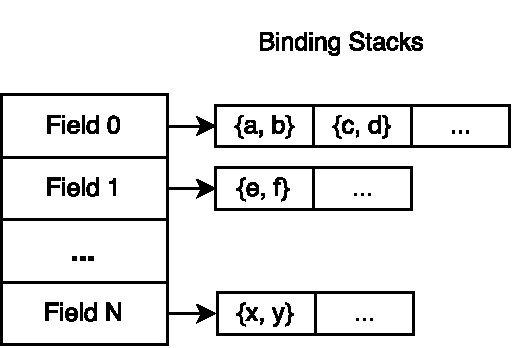
\includegraphics[scale=0.75,natwidth=203,natheight=298]{context}
\caption{The binding environment inside a context used to store the length and offset of fields, or the offset of headers. On the left, fields one through sixteen represent the fields that can be extracted. Each field maintains a binding list (stack). Each element in the binding list is a binding which stores the offset and length where each instance of that field can be found in the packet. }
\label{fg:ContextEnv}
\end{figure}

Figure \ref{fg:ContextEnvWorking} demonstrates how data is stored in the context as it is being decoded. The example is a packet which contains an encapsulated IPv4 header commonly used in IP tunneling. In the ethernet decoding stage which extract the \texttt{src}, \texttt{dst}, and \texttt{type} field are extracted and stored in the context. Next we determine that IPv4 follows based on the \texttt{type} field. We extract IPv4 \texttt{dst} and \texttt{protocol}. The \texttt{protocol} field tells us we have another IPv4 header after the current one. We move to decode that and once again we extract IPv4 \texttt{dst} and \texttt{protocol}. Note how the new values of IPv4 are pushed on top of the binding stack. Any further usage of those fields will use the latest values extracted for those fields. Keep in mind that this means any usage of the first set of IPv4 \texttt{dst} and \texttt{protocol} must occur before the decoding of the second IPv4 header.\

\begin{figure}
TODO: Make an image for this.
\caption{A context environment in action during runtime.}
\label{fg:ContextEnvWorking}
\end{figure}

The \textbf{action set} is the other major data structure contained within the context. The action set is a set of actions which have been written to the context for deferred execution using a \texttt{write action} (see Section \ref{action_tut}). Upon reaching a designated egress port, the action set is executed right before the packet is output.

\section{Table Stage} \label{table_desc}

Table stages handle matching against extracted fields, i.e. classification, and perform a sequence of desired actions on like-classified packets. This is done through a mechanism known as a flow table \cite{openflow_spec}.

A \textbf{flow table} is composed of a set of \textbf{flow entries}. A flow entry is composed of \textbf{match fields}, a \textbf{priority}, a set of \textbf{actions}, and miscellaneous additional data. Each table specifies a set of key fields that together make up a \textbf{key} for that table. For each key field, each flow entry has a corresponding value, known as a \textbf{match field}, such that every flow entry in the table is uniquely identified by its match fields and its \textbf{priority}.

When a packet reaches a table matching stage, the fields comprising the table's key are extracted from the context. Lookup into the table retrieves all flow entries whose match fields can correctly match the field values from the packet. The flow entry whose priority is highest is selected. The \textbf{actions} of the flow entry are executed on the packet.

If no such flow entry matches against the packet's field values, the \textbf{miss case} flow entry is applied to the packet instead. Flow entries can be user defined. By default, a miss in a table results in the packet being dropped. Miss cases always have the lowest possible priority amongst flow entries and each match field can be considered a wildcard.

The mechanic of table matching is not distinctly different from those of relational or SQL tables. In fact, Frenetic, another packet processing language, uses SQL-inspired syntax to classify flows \cite{frenetic_paper1}. If we make this comparison, a flow table is analogous to a SQL table, the concept of a key is the same for both, and a flow entry is analogous to a tuple in a SQL table. Each packet and its fields constitute the actual "query" into the table.

\section{Pipeline Composition} \label{pipeline_comp_desc}

Kinds of processing stages can be interleaved together in any order within the pipeline. This means that Steve is capable of supporting different packet processing paradigms found in other research such as POF and P4. With the Steve pipeline specification language a user can specify that a pipeline does:

\begin{enumerate}
\item \textbf{A full decode of the packet followed by a sequence of tables.} Packets coming to the pipeline have all necessary headers and fields are decoded and saved in the runtime context first. The packet is then dispatched to the first table in the pipeline. From there, matched flows within the tables dictate which table the packet is sent to next or which port the packet is forwarded to.
\item \textbf{A chain of partial decodes and table lookups.} Packets coming to the pipeline get partially decoded and dispatched to a table. The flow within that table could carry the packet to another table, another decoder, or forward it out of the network. The pipeline in this case in a chain of alternating sequences of decoding stages and table matching stages.
\item \textbf{Only decodes.} In some special cases, it may not even be necessary to go to a table matching stage. It may be possible to make a decision about the packet’s ultimate destination immediately upon evaluating a certain field within the packet using a simple conditional statement (if-statement, if-else statement, etc). Therefore, decoding stages also support the range of actions supported by flow entries, which can include outputting packets to a port or dropping it.
\end{enumerate}

Upon entering the pipeline, a packet must first go through at least one decoding stage before moving to the next processing stage. From there, the packet flows from one stage of the pipeline to the next. With each stage, certain conditions are evaluated which will determine where the packet must flow next. Finally, the packet will exit the pipeline either through a port(s) or by being dropped and discarded.

\chapter{Tutorial} \label{tutorial}

This chapter provides a tutorial on the syntax of Steve and using its language features. Steve's primary focus is to provide language features for declaring, specifying, and constructing the pipeline processing stages described in Chapter \ref{pipeline_model}. This chapter will explain how to represent packet headers, how to write decoding stages, how to write table stages, and how to use actions.

Throughout this chapter there be small semantic details mentioned when necessary. For complete details on the semantics of Steve, see the User's Guide in Chapter \ref{users_guide}.

For a complete reference of all Steve syntax, see Appendix \ref{ap:a}.

\section{Layouts} \label{layout_tut}

Before pipeline processing stages can be written, a \textbf{layout} is used to describe the physical structure of a packet header, i.e. what fields they have and the respective lengths of those fields. Figure \ref{fg:layout_syntax} provides the syntax for layout declarations in BNF notation.

A \textbf{layout declaration} is composed of a sequence of \textbf{field declarations}. Each field declaration corresponds to a field in a header. The type of each field declaration defines the length of the corresponding field in a header. Each field declaration in a layout must be written in the same order with which the field appears in a real instance of the header. If the ordering does not match, layouts will not function correctly during decoding stages. 

\begin{figure}
\begin{mdframed}
\begin{grammar}

<layout-decl> ::=
\textbf{layout} <layout-name> 
\textbf{\{}
	<field-decl> +
\textbf{\}}

<field-decl> ::=
<field-name> \textbf{:} <type> \textbf{;}

<type> ::=
<scalar-type>
\alt <layout-type>

<scalar-type> ::= <integer-type>

<integer-type> ::=
\textbf{int} [ \textbf{(} <integer-literal> \textbf{)} ]
\alt \textbf{uint} [ \textbf{(} <integer-literal> \textbf{)} ]

<layout-type> ::=
<layout-decl-id>

\end{grammar}
\end{mdframed}
\caption{Layout syntax for Steve in BNF.}
\label{fg:layout_syntax}
\end{figure}

A field declaration within a layout is limited to being one of two different types. The first of these types is scalar type (most often a signed/unsigned integer type). Integer types can be given with an optional bit-length precision, with the default being 32-bits if no precision is specified. This bit-length precision is used to determine the length of the field. An example of a layout corresponding to the ethernet header \cite{eth_std} can be seen in Figure \ref{fg:ethernet_layout_ex}. The \texttt{src} and \texttt{dst} fields are 48-bits, or 6 bytes, long. The \texttt{type} field is 16-bits, or 2 bytes, long.

\begin{figure}
\begin{lstlisting}
layout eth
{
  dst  : uint(48);
  src  : uint(48);
  type : uint(16);
}
\end{lstlisting}
\caption{An example of how the ethernet header is written in Steve.}
\label{fg:ethernet_layout_ex}
\end{figure}

The second supported type is layout type. This allows layouts to be nested together in case a programmer must deal with a header with structures nested inside them. In this case, a field declaration is used whose type is given as the identifier to layout declaration. Figure \ref{fg:nested_layout_ex} gives a trivial example of nested layouts.

\begin{figure}
\begin{lstlisting}
layout eth
{
  dst  : uint(48);
  src  : uint(48);
  vlan_tag : vlan;
  type : uint(16);
}

layout vlan
{
  tpid : uint(16);
  tci  : uint(16);
}
\end{lstlisting}
\caption{An example of a layout being nested inside another layout.}
\label{fg:nested_layout_ex}
\end{figure}

Keep in mind that a layout, though similar to a class, is not a class. Objects of layout type can never be created, they cannot contain member functions, and their fields must all be of scalar or layout type. Layouts are use to determine two things: what the offset of a given field is relative to the beginning of the header and the length of the field. These two pieces of information are important during decoding stages where these fields are extracted. In this way, layouts more closely translate to extraction rules used during the decoding process. 

The primary reason for this differentiation in Steve are dynamically-sized fields in packet headers. Headers potentially have fields whose memory size is predicated upon some value discovered during runtime. These fields are said to have \textbf{dynamically sized type}. Some examples of this are the \texttt{options} fields in IPv4, IPv6, and TCP headers. Consider that when objects of any type are constructed, stack space must be allocated for them. Except, it is impossible to stack allocate an object whose size is not known during compilation without some hint about its maximum size. Such objects can only be heap allocated, which Steve does not currently support. 

Furthermore, accessing these dynamically-sized fields, recovering their values, and performing operations on them would have to be done through special pointers to ensure the safety of such operations. For further details on layout limitations, refer to Section \ref{layout_guide} in the User's Guide.

Steve does not currently support dynamically sized types. This is a language feature that will eventually be added, but is outside the scope of this thesis. Because of this, fields whose lengths are dynamic cannot currently be declared, extracted, nor used. 

An IPv4 header example can be seen in Figure \ref{fg:ipv4_layout_ex}. Note that the \texttt{options} field is skipped due to the lack of dynamically sized types. Also note that Steve does not support non-byte aligned data types, and thus the precision of all integers are multiples of 8. Fields which are non-byte aligned must be merged to byte alignment and recovered using arithmetic operations (see Figure \ref{fg:assign_arith_ex} in Section \ref{decoder_tut} for an example). 

\begin{figure}
\begin{lstlisting}
layout ipv4
{
  version_ihl : uint(8);
  dscp_ecn    : uint(8);
  len         : uint(16);
  id          : uint(16);
  fragment    : uint(16);
  ttl         : uint(8);
  protocol    : uint(8);
  checksum    : uint(16);
  src         : uint(32);
  dst         : uint(32);
}
\end{lstlisting}
\caption{An example of how the IPv4 header is written in Steve. Note that the "options" field is not included because Steve does not currently support extraction or usage of dynamic length fields.}
\label{fg:ipv4_layout_ex}
\end{figure}


\section{Decoders} \label{decoder_tut}

\textbf{Decoders}, also referred to as decoding stages in the pipeline processing model,  are special purpose functions used to handle decoding and extracting fields in a given header. By chaining multiple decoders together, a user can construct a set of functions used to parse an entire packet. \textbf{Decoder declarations} are Steve's way of defining decoding stages. Figure \ref{fg:decoder_syntax} presents the syntax used to write decoders. Decoder declarations provide users the ability to:

\begin{itemize}
\item Declare which header is being decoded and which fields to extract from it.
\item Perform arithmetic and logical operations on fields.
\item Perform actions on the header. See Section \ref{action_tut} for examples of action usage.
\item Decide what processing stage comes next. Either the next header is determined and the packet is dispatched to that decoding stage, or the packet is dispatch to table matching.
\end{itemize}

\begin{figure}
\begin{mdframed}
\begin{grammar}

<decoder-decl> ::=
\textbf{decoder} <decoder-name> [\textbf{start}] 
\textbf{(} <layout-id> \textbf{)}
<block-statement>

<extract-decl> ::=
\textbf{extract} <field-name> \textbf{;}

<rebind-decl> ::=
\textbf{extract} <field-name> \textbf{as} <field-name-expr> \textbf{;}

<field-name> ::=
<layout-id> \textbf{.} <field-id>
\alt <field-name> \textbf{.} <field-id>

<field-access-expr> ::=
<layout-id> \textbf{.} <field-id>
\alt <field-access-expr> \textbf{.} <field-id>

\end{grammar}
\end{mdframed}
\caption{Decoder syntax for Steve in BNF.}
\label{fg:decoder_syntax}
\end{figure}

\subsection{Extractions} \label{decoder_extract_tut}

The primary goal of decoders is to extract fields from headers. Assume we wanted to write a decoder to extract the \texttt{src} and \texttt{dst} fields from an ethernet header. Remember, Steve allows for the partial decoding of packets, so if we do not need a field, in this case \texttt{type}, its not necessary to extract it. 

First, a layout for the ethernet header must be defined. In this case, the layout defined in Figure \ref{fg:ethernet_layout_ex} can be used. This layout will be used to determine the offset (location) and length of each field in the header during decoding. More details on this process can be found in Section \ref{decoder_guide}. 

After that, we can proceed to writing the decoder declaration. Figure \ref{fg:extract_ex} demonstrates how the extraction is written. We give this decoder declaration the name \texttt{eth\_decode} and specify the layout used to decode in the parenthesis following the name (in this case \texttt{eth}). A decoder can only extract fields from a header defined by this layout. If an attempt is made to extract a field from a different header a compiler error is emitted. The optional \texttt{start} keyword is attached to this decoder to denote that this decoder is the first stage in the pipeline. Ethernet is the most commonly used data link layer protocol, making it the most common header to start with. There can only be one starting decoder. 

To extract a field, the programmer writes an \textbf{extract declaration} which requires that a field be specified using a \textbf{field name}. A field name is used to refer to a field of a layout. For example \texttt{eth.dst} refers to the \texttt{dst} field of the \texttt{eth} layout.  Note that this is distinctly different from member access as the \texttt{eth} layout is not an object. 

The first extract declaration (\texttt{extract eth.dst;}) says that the decoder extracts the \texttt{dst} field of the \texttt{eth} header. The second extract declaration (\texttt{extract eth.src;}) says that the decoder extracts the \texttt{src} field of the \text{eth} header. 

\begin{figure}
\begin{lstlisting}
decoder start eth_decode(eth)
{
  extract eth.dst;
  extract eth.src;
  // More code to follow...
}
\end{lstlisting}
\caption{An example of how to extract \texttt{src} and \texttt{dst} fields from the ethernet header using a decoder. Note we do not extract the \texttt{type} field here.}
\label{fg:extract_ex}
\end{figure}

\subsection{Accessing Extracted Fields} \label{decoder_access_tut}

After extracting a field from a header, a programmer will almost certainly want to use the field in some kind of operation whether that be arithmetic or logical. To use the \textit{value} of an extracted field, a programmer uses a \textbf{field access expression}. Field access expressions have the same grammar as field names, but they can be used wherever any expression is valid. The behaviour of field access expressions is similar to how the name of a variable can be used to mean the value stored in that variable in C-like languages.

Figure \ref{fg:access_ex} demonstrates how the value of extracted fields can be used in Steve. In this scenario, we extract \texttt{eth.type} and use the value as a condition in a C-like if-else statement. We use this if-else statement to determine what the \texttt{type} field means. The IEEE ethernet standard says that if the \texttt{type} field is greater than or equal to hexadecimal \texttt{0x600}, then the value of the field is used to determine the kind of header encapsulated by the ethernet header \cite{eth_std}. Otherwise, if the \texttt{type} field is less than hexadecimal \texttt{0x05dc}, the field refers to the length of the ethernet frame.

\begin{figure}
\begin{lstlisting}
decoder start eth_decode(eth)
{
  extract eth.type;
  
  // Using a field access expression 
  // with logical operator >=
  if (eth.type >= 0x600)
  {
    // Then this is determines what
    // header comes next.
  }
  // Using a field access expression 
  // with logical operator <=
  else if (eth.type <= 0x05dc)
  {
    // Then this is the length field.
  }
  // ...
}
\end{lstlisting}
\caption{An example of accessing a field using the field access expression in an if-else statement.}
\label{fg:access_ex}
\end{figure}

Field access expressions can also be used in arithmetic operations, bitwise operations, and can be stored and assigned to local variables. Figure \ref{fg:assign_arith_ex} demonstrates how this can be done using an IPv4 decoder as an example. First it's shown that it's possible to assign the value of the header's \texttt{len} field to a local variable named \texttt{pktlen}. Next the example shows how to recover \texttt{ihl} and \texttt{version} from a single field (to deal with the limitation of only supporting byte-aligned fields). Note that it is possible to use bitwise and shift operations on fields as well. After that, the example demonstrates subtraction on the \texttt{ipv4.len} field to determine what the time-to-live will be after the packet leaves the current device.

\begin{figure}
\begin{lstlisting}
decoder ipv4_decode(ipv4)
{
  extract ipv4.len;
  extract ipv4.version_ihl;
  extract ipv4.ttl;
  
  // We can assign to variables
  var pktlen : uint = ipv4.len;
  
  // We can perform bitwise operations.
  var ihl : uint(8) = ipv4.version_ihl & 0x0f;
  // We can also perform shifts.
  var version : uint(8) = (ipv4.version_ihl & 0xf0) >> 4;
  
  // Determine what the Time-to-Live is after this
  // device finishes with the packet.
  var next_ttl : uint = ipv4.ttl - 1;
  
  // ...
}
\end{lstlisting}
\caption{Using arithmetic operations, bitwise operations, and variable assignment with fields in a Steve program.}
\label{fg:assign_arith_ex}
\end{figure}

Field access expressions do have a number of limitations. A field access expression can only be used \textit{after} an extract declaration is used for that field. After all, it is impossible to recover the value of a field which has not been extracted. They cannot be used in decoders which have not extracted that field. A decoder focuses on exactly one header and has no knowledge of previous headers or extractions. Field access expressions cannot be assigned to. To modify the value of a field in a header, an action must be used (see Section \ref{action_tut}). Figure \ref{fg:bad_access_ex} shows incorrect usage of field access expressions.

\begin{figure}
\begin{lstlisting}
decoder start eth_decode(eth)
{
  // Error: Cannot use eth.type before its extracted.
  if (eth.type >= 0x600) 
  {
    // Do something...
  }
  
  extract eth.type;
  
  // Error: Cannot assign to a field this way.
  eth.type = 0x800;
  // ...
}

decoder ipv4_decode(ipv4)
{
  // Error: eth.type was not extracted by this decoder.
  if (eth.type == 0x800)
  {
    // Do something...
  }
  // ...
}
\end{lstlisting}
\caption{An example of incorrect field access.}
\label{fg:bad_access_ex}
\end{figure}

\subsection{Moving to Other Stages} \label{decoder_next_tut}

As mentioned earlier, decoding and table matching stages can be chained together in a number of flexible ways. A decoder can transition a packet to another decoder, it can transition to a table matching stage, or it can forward/drop the packet. Its up to the programmer to decide which is appropriate. Every stage in the pipeline is \textbf{required} to do one of these three.

To transition to another decoding stage, a \texttt{decode} statement is used. To transition to a table matching stage, a \texttt{goto} statement (not to be confused with a C-like \texttt{goto}) is used. 

Figure \ref{fg:transition_ex} demonstrates how to move from a decoder to a decoder, from a decoder to a table, then from a table to another decoder. There are a few important things to note. First, inside the if-statement, we have a match statement. A match statement is similar to a C-like switch statement in every way, except there is an implied \texttt{break} at the end of every case. From the \texttt{eth\_decode} decoder, we move to the \texttt{ipv4\_decode} decoder if the value of \texttt{eth.type} is \texttt{0x800}. 

\begin{figure}
\begin{lstlisting}
decoder start eth_decode(eth)
{
  extract eth.type;
  if (eth.type >= 0x600) 
  {
  	// Check to see if the next header is ipv4.
    match (eth.type)
    {
      case 0x800: decode ipv4_decode;
    }
  }
  
  // Do something else...
}

decoder ipv4_decode(ipv4)
{
  extract ipv4.version_ihl;
  extract ipv4.dst;
  extract ipv4.protocol;
  
  var ihl : uint(8) = ipv4.version_ihl & 0x0f;
  
  goto t1 advance ihl;
}

exact_table t1(ipv4.dst, ipv4.protocol)
{
  {0x0a_16_21_2c, 0x11} ->
  {
    // Assuming a udp decoder exists named "udp_decode"
    decode udp_decode;
  }
  
  miss -> { drop; }
}
\end{lstlisting}
\caption{An example of using \texttt{decode} and \texttt{goto} to transition between stages.}
\label{fg:transition_ex}
\end{figure}

In the \texttt{ipv4\_decode} decoder, fields get extracted as usual. A \texttt{goto} statement is used to move the packet from the decoder to a table matching stage name \texttt{t1}. However, the \texttt{advance ihl} clause added is not typical. By default, when transitioning from a decoding stage to another stage (either by using \texttt{decode} or \texttt{goto}), the "view" of the current header automatically shifts to a "view" of the next header. This shift implicitly moves the "view" over by the length of the current header. However, with \textbf{all headers of dynamic length} such as IPv4, the shift has to be done explicitly through the advance clause. Further details about how this "view" and shifting process work can be found in Chapter \ref{users_guide} Section \ref{decoder_guide}.

From table \texttt{t1}, if the packet's \texttt{ipv4.dst} and \texttt{ipv4.type} fields match certain values, the packet is sent to a UDP decoder. Otherwise, the miss case is triggered and the packet gets dropped. A tutorial on using tables can be found in Section \ref{table_tut}. 

\section{Tables} \label{table_tut}

The next stage to explore is the table matching stage. Table matching allows the programmer to \textbf{classify} packets and perform a specific sequence of actions on like-classified packets. This is done through a mechanism known as a flow table. A \textbf{flow table} is composed of a set of \textbf{flow entries}. A flow entry is a mapping of unique keys to flows. A \textbf{key} is defined as a field value or unique combination of field values such that every key in the flow table can be uniquely identified. A \textbf{flow} is defined as a sequence of actions (operations that can affect a packet, its action set, or the pipeline).

There are three commonly used types of flow tables: \textbf{exact}, \textbf{prefix}, and \textbf{wildcard} matching tables. Steve currently only supports the exact match table. 

With an exact match table, each field in the packet must \textit{exactly} match the corresponding field value in a flow entry's key for the packet to match that flow entry. If a flow entry match is found by the table, the flow is executed on the packet.

Figure \ref{fg:table_syntax} provides the syntax for writing tables and flow entries in Steve. Tables are written using \textbf{table declarations} and flow entries are written using \textbf{flow declarations}.

\begin{figure}
\begin{mdframed}
\begin{grammar}
<table-decl> ::=
\textbf{table} <table-name> \textbf{(} <key-decl-sequence> \textbf{)} 
[ <requires-clause> ]
\textbf{\{} 
<flow-decl> + 
\textbf{\}}

<key-decl> ::=
<layout-id> \textbf{.} <field-id>
\alt <key-decl> \textbf{.} <field-id>
\alt \textbf{in\_port}
\alt \textbf{in\_phys\_port}

<requires-clause> ::=
\textbf{requires} \textbf{(} <field-name-sequence> \textbf{)}

<flow-decl> ::=
<properties-block>
\textbf{\{} [<expr-sequence>] \textbf{\}} \textbf{-\textgreater}
\textbf{\{} 
<action> +
\textbf{\}}
\alt <miss-flow-decl>

<properties-block> ::=
\textbf{[} <property-sequence> \textbf{]}

<property> ::=
<property-kind> \textbf{=} <expr>

<property-kind> ::=
\textbf{timeout}
\alt \textbf{egress}

<miss-flow-decl> ::=
\textbf{miss} \textbf{-\textgreater}
\textbf{\{} 
<action> +
\textbf{\}}
\end{grammar}
\end{mdframed}
\caption{Table syntax for Steve in BNF.}
\label{fg:table_syntax}
\end{figure}

To write a complete exact match table, the programmer must specify 1) what fields are being used for classification, 2) what additional fields need to be extracted by a decoder before reaching the table, and 3) a set of flow entries. 

A basic static routing table can found in Figure \ref{fg:basic_table_ex}. This code declares a table named \texttt{route} which matches on \texttt{ipv4.dst} and \texttt{ipv4.protocol}. In addition, it requires that \texttt{ipv4.ttl} be extracted. All fields which are part of the table's key are implicitly required to be extracted. Assume that the system has some preconfigured ports with the configuration given in \texttt{p1} and \texttt{p2}. We define two initial flow entries and a miss case for when packets cannot be classified as either entry. 

The first flow entry matches packets whose IP destination address is 69.89.31.226 and whose data protocol is UDP (0x11). The first flow entry matches packets whose IP destination address is 10.24.200.50 and whose data protocol is also UDP.

\begin{figure}
\begin{lstlisting}

// Open sockets with given configuration.
Port p1 = ":5000"
Port p2 = ":5001"

exact_table t1(ipv4.dst, ipv4.protocol)
	requires (ipv4.ttl)
{
  // Flow Entry #1
  // This brace enclosed list defines the key.
  // 0x45_59_1f_e2 == 69.89.31.226
  { 0x45_59_1f_e2, 0x11 } ->
  // This block defines the sequence of actions.
  {
    set ipv4.ttl = ipv4.ttl - 1;
    // output the packet to port p1
    output p1;
  }
  
  // Flow Entry #2
  // 0x0a_18_c8_32 == 10.24.200.50
  {	0x0a_18_c8_32, 0x11 } ->
  {
    set ipv4.ttl = ipv4.ttl - 1;
    // output the packet to port p2
    output p2;
  }
  
  // Miss Case
  miss ->
  {
    // drop the packet
  }
}
\end{lstlisting}
\caption{An example of a simple static routing table which matches on two fields.}
\label{fg:basic_table_ex}
\end{figure}


\section{Actions} \label{action_tut}

Actions are used to change packets, action sets, and the pipeline. Steve supports ten actions with more anticipated in the future.

\begin{figure}
\begin{mdframed}
\begin{grammar}
<action-stmt> ::=
<decode-action>
\alt <goto-action>
\alt <output-action>
\alt <drop-action>
\alt <flood-action>
\alt <clear-action>
\alt <set-field-action>
\alt <insert-flow-action>
\alt <remove-flow-action>
\alt <raise-action>
\alt <write-action>

<decode-action> ::=
\textbf{decode} <decoder-decl-id> \textbf{;}

<goto-action> ::=
\textbf{goto} <table-decl-id> \textbf{;}

<output-action> ::=
\textbf{output} <port-expr> \textbf{;}

<drop-action> ::= \textbf{drop;}

<flood-action> ::= \textbf{flood;}

<clear-action> ::= \textbf{clear;}

<set-field-action> ::= \textbf{set} <field-access-expr> \textbf{=} <expr> \textbf{;}

<insert-flow-action> ::= \textbf{insert} <flow-decl> \textbf{into} <table-id> \textbf{;}

<remove-flow-action> ::= \textbf{remove} \textbf{\{} [ <expr> + ] \textbf{\}}
\textbf{from} <table-id> \textbf{;}

<raise-action> ::= \textbf{raise} <event-id> \textbf{;}

<write-action> ::= \textbf{write} <action-stmt>

\end{grammar}
\end{mdframed}
\caption{Action syntax for Steve in BNF.}
\label{fg:action_syntax}
\end{figure}

\section{Events} \label{event_tut}

\section{Examples} \label{examples_tut}
\chapter{User's Guide} \label{users_guide}

This chapter will explore the "anatomy" of Steve. It will dissect the semantics and limitations for each language feature. This chapter expects that the user has read the Tutorial and has a basic understanding of Steve. Some semantics from the Tutorial chapter will be repeated and expanded.

This section shall elaborate on the conventional and illegal uses of the language. In many cases, the syntax used by the programmer has been abstracted away from much grittier details via "compiler magic". This chapter shall also elaborate on these inner mechanics.

Steve makes guarantees about the logical correctness and safety of pipeline stage composition. This section will detail how the Steve language enforces those guarantees and prove that these guarantees can be correctly enforced.

\section{Identifiers} \label{identifiers_guide}

An \textit{identifier} is an arbitrarily long sequence of characters. Supported characters include uppercase Latin letters (\texttt{A - Z}), lowercase Latin letters (\texttt{a - z}), digits (\texttt{0 - 9}), and underscores (\_). A valid identifier must begin with a non-digit character. Identifiers are case sensitive. The grammar of identifiers is as follows:

\begin{minip}
\begin{grammar}
<identifier> ::= <letter><identifier-characters>+

<identifier-character> :: <letter>
\alt <digit>
\alt \textbf{\_}

<letter> ::= "A" | "B" | "C" | "D" | "E" | "F" | "G"
       | "H" | "I" | "J" | "K" | "L" | "M" | "N"
       | "O" | "P" | "Q" | "R" | "S" | "T" | "U"
       | "V" | "W" | "X" | "Y" | "Z" | "a" | "b"
       | "c" | "d" | "e" | "f" | "g" | "h" | "i"
       | "j" | "k" | "l" | "m" | "n" | "o" | "p"
       | "q" | "r" | "s" | "t" | "u" | "v" | "w"
       | "x" | "y" | "z"

<digit> ::= 0 | 1 | 2 | 3 | 4 | 5 | 6 | 7 | 8 | 9
\end{grammar}
\end{minip}

Identifiers are subject to the following limitations:

\begin{itemize}
\item Identifiers which are keywords cannot be used for other purposes (see Section \ref{keyword_guide}).

\item Identifiers beginning with double underscores (\_\_) or an underscore followed by a capital letter (ex. \_F) are reserved by the compiler for internal identifiers.
\end{itemize}

Identifiers can be used as \textit{names} for \textit{entities}. An entity is a value, object, reference, function, layout, layout field, decoder, table, flow entry, port, event, extraction. In the Steve grammar, identifiers being used as names for a kind of declarations shall have the form \grd{kind}{name}, where \texttt{\textit{kind}} shall be the declaration kind. For example, a decoder name would be represented in the grammar as \grd{decoder}{name}.

Identifiers that name a variable, function, decoder, table, or port can be used as an expression. In this case, the identifier becomes an \textit{identifier expression}. Identifier expressions refer to a declaration. In cases where identifier expressions refer to object declarations (see \ref{object_guide}) a \textit{reference} to \textit{value} conversion is applied (see Section \ref{reftoval_conv}. In the Steve grammar, identifier expressions shall have the form \grd{kind}{id}, where \texttt{\textit{kind}} shall be the declaration kind. For example, an identifier to a variable would be represented in the grammar as \grd{variable}{id}.

\section{Keywords} \label{keyword_guide}

A number of identifiers in Steve are reserved as \textit{keywords}. The meaning and semantics of these identifiers cannot be changed. A list of Steve keywords can be found in Figure \ref{keywords_table}.

\begin{figure} [ht]
{\ttfamily
\begin{tabular*}{\textwidth\noindent}{@{\extracolsep{\fill}} l l l l l}
bool   & break   & char    & continue & def  \\
if     & else    & foreign & int      & uint \\
return & struct  & this    & var      & while \\
match  & case    & layout  & decoder  & decode \\
start  & extract & as      & exact\_table & requires \\
miss   & Port    & goto    & output   & write \\
drop   & flood   & clear   & set      & insert \\
remove & into    & from    & event    & raise \\
in\_port & in\_phys\_port & all & controller & reflow \\
advance & egress & struct & char
\end{tabular*}
}
\caption{Steve reserved keywords. Note that Steve reserves the right to make any identifiers keywords in future versions.}
\label{keywords_table}
\end{figure}

\section{Field Name} \label{field_name_guide}

\textit{Field names} are special, \textit{qualified} names which refer to field declarations made within a layout declaration. Field names have the form:

\begin{minip}
\begin{grammar}
<field-name> ::=
<layout-id> \textbf{.} <field-id>
\alt <field-name> \textbf{.} <field-id>
\end{grammar}
\end{minip}

In the first form \grd{layout}{id}.\grd{field}{id}, or more succinctly \texttt{E1.E2}, \texttt{E1} must be a valid identifier to a layout declaration. \texttt{E2} must be found in the layout scope of \texttt{E1} using a qualified name lookup (see \ref{qlfd_lookup}).

In the second form \grd{field}{name}.\grd{field}{id}, or more succinctly \texttt{E1.E2}, \texttt{E1} must be a valid field name which refers to a field declaration whose type, \texttt{T}, is layout type (see \ref{layout_type_guide}). \texttt{E2} must be found in the layout scope of the layout declaration declaring type \texttt{T} using qualified name lookup.

In both forms, \texttt{E1} is referred to as the \textit{container} and \texttt{E2} is referred to as the \textit{contained field}.

The \textit{containing layout identifier} is the phrase used to mean the leftmost identifier in a field name.

Field names used as expressions become \textit{field access expressions} (see \ref{field_access_expr_guide}). Field access expressions may be used to refer to the value of the last extraction of that field name.

\section{Scope} \label{scope_guide}

Steve scope semantics borrow heavily from C++ scope semantics \cite{cpp_std}. \textit{Declarations} are used throughout program text to introduce \textit{names}. Names are \textit{identifiers} used to identify \textit{entities} (see \ref{identifiers_guide}). A \textit{name} is only \textit{valid} within parts of program text called the \textit{scope} of that name. A particular name is only considered valid if an \textit{entity} with that name can be found using an \textit{unqualified name lookup} (see \ref{unqlfd_lookup}).

\subsection{Global Scope} \label{global_scope}

The outermost part of program text where declarations can be made is known as \textit{global scope}. All declarations made at global scope are said to be \textit{global declarations} and their names are said to be \textit{global names}.

Global names are valid at any point in the program. Steve does not require forward declarations.

Two different declarations of the same name shall not be made at global scope. Any attempts to do this shall produce a compiler error.

\subsection{Block Scope} \label{block_scope}

Blocks are portions of program text which can have their own local declarations. The beginning of a block is delimited by the left-brace (\{) and the end of a block is delimited by the right-brace (\}). A declaration made within a block is in \textit{block scope} and is \textit{local} to that block.

Two different declarations of the same name cannot be made inside the same block. Any attempts to do this shall produce a compiler.

Scopes can be nested. In this case, the inner scope is said to be the \textit{enclosed} scope, and the outer scope is said to be the \textit{enclosing} scope. The same name can be declared in the enclosing scope, and again in one or more enclosed scopes. The same is true for further nested scopes within the enclosed scope. If this happens, the scope of the outer declaration is its typical scope excluding program text of the enclosed scope. Unqualified name lookup (see \ref{unqlfd_lookup}) shall be used to unambiguously determine which declaration the name refers to.

The statements \texttt{if}, \texttt{while}, \texttt{match} all implicitly introduce a block.

%Here, it is useful to talk about a concept called \textit{potential scope}, similarly found in C++ \cite{cpp_std}. The scope of a declaration is the same as its potential scope. The only exception is if there are two or more declarations of the same name in the same potential scope. In this case, the actual scope of a declaration is its potential scope excluding the potential scope of the inner declarative region.

Blocks found in the program text at global scope (i.e. function bodies, layout bodies, decoder bodies, etc) introduce block scopes which are nested in global scope.

For example, in the following example, the name \texttt{i} is declared twice. The scope of the first \texttt{i} is global scope and includes the entire example excluding the block between the first left-brace (\texttt{\{}) and the closing right-brace (\texttt{\}}). The scope of the second \texttt{i} begins immediately after its declaration and ends at the the closing right-brace (\texttt{\}})

\begin{minip}
\begin{lstlisting}
var i : int = 0;
def f() -> int
{
	var i : int = 1;
	var j : int = 2 + i;
	return j; // Result here shall be 3.
}
\end{lstlisting}
\end{minip}

\subsection{Function Scope} \label{function_scope}

The body of a function declaration (see \ref{function_guide}) is its \grd{block}{statement} which introduces a block. All names introduced by a \grd{parameter}{declaration} in a function declaration's \grd{parameter}{sequence} have an effective scope starting at the beginning of the block.

\subsection{Decoder Scope} \label{decoder_scope}

The body of a decoder declaration (see \ref{decoder_guide}) is its \grd{block}{statement} which introduces a block. Declarations made inside this block are said to have \textit{decoder scope}.

\subsection{Table Scope} \label{table_scope}

A table declaration (see \ref{table_guide}) has a body given by \grd{table}{initializer} which introduces a block. Declarations made inside this block are said to be in \textit{table scope}.

All field names given by a \grd{key}{declaration} within \grdd{key}{declaration}{sequence} extends the scope of those field names into the table scope. Those field names are names declared via extract declaration (see \ref{extract_guide}) in a prior stage declaration of the pipeline. Field names declared via \grdd{key}{declaration} are valid and can be extended into the table scope if and only if \textit{requirements satisfaction} (see \ref{requirements_guide}) determines that field is satisfied.

All field names given by the \grd{requires}{clause} extends the scope of those field names into the table scope. \textit{Requirement satisfaction} is used to check whether or not those names are valid and can be extended.

In the following example, we declare two decoders; \texttt{ipv4\_d} has extract declarations for field names \texttt{ipv4.type} and \texttt{ipv4.ttl}; \texttt{udp\_d} has extract declarations for \texttt{udp.dst\_port}.

\begin{minip}
\begin{lstlisting}
decoder ipv4_d(ipv4)
{
	extract ipv4.type;
	extract ipv4.ttl;
	// ...
	decode udp;
}

decoder udp_d(udp)
{
	extract udp.dst_port;
	// ...
	goto t1;
}
\end{lstlisting}
\end{minip}

We go to table \texttt{t1} from \texttt{udp\_d}. Table \texttt{t1} has the key declarations \texttt{ipv4.type} and \texttt{udp.dst\_port} introduce those field names into table scope. What they are actually doing is \textit{extending} the scope of those names from the respective extract declarations into the scope of \texttt{t1}. The same \textit{scope extension} is applied to \texttt{ipv4.ttl}.

\begin{minip}
\begin{lstlisting}
exact_table t1(ipv4.type, udp.dst_port)
	requires(ipv4.ttl)
{
	{ 0x01, 80 } ->
	{
		// The ipv4.type field name is valid here.
		set ipv4.type = 0x02;
		// The udp.dst_port field name is valid here.
		set udp.dst_port = 88;
		// The ipv4.ttl field name is valid here.
		set ipv4.ttl = ipv4.ttl - 1;
	}
}
\end{lstlisting}
\end{minip}

\subsection{Flow Entry Scope} \label{flow_scope}

A flow declaration has a body given by \grd{flow}{body} which introduces a block. Declarations made in this block are said to have \textit{flow entry scope}. If a flow declaration is part of a table declaration's \grd{table}{initializer}, the flow declaration has table scope. The flow entry scope is nested inside table scope.

If a flow declaration is part of an \texttt{insert} action, the body is treated as if it were nested inside the table scope of the table it is being inserted into.

Names found in the \grd{properties}{block} follow regular scope semantics. That is, all names which are normally valid at the point where the \grd{properties}{block} appears in the program text are valid inside the \grd{properties}{block}. However, these names may not be valid for the \grd{flow}{body} in the case of an \texttt{insert} action.

In the following example, the name \texttt{x} is valid in the properties block, but not in the body of the flow.

\begin{minip}
\begin{lstlisting}
event e1
{
	var x : int = 100;
	insert
	[timeout = x] // 'x' is valid here.
	{ x } -> // 'x' is also valid here.
	{
		// Error: The name 'x' is not valid here.
		set eth.type = x + 1;
		// However, the field name 'eth.type' is valid
		// because the flow body is treated as if nested
		// inside the scope of table 't1', whose key declaration
		// 'eth.type' makes the field name valid.
		flood;
	}
	into t1;
}

exact_table t1(eth.type) { }
\end{lstlisting}
\end{minip}

\subsection{Event Scope} \label{event_scope}

The body of an event declaration (see \ref{event_guide}) is a \grd{block}{statement} which introduces a block. All field names given by the \grd{requires}{clause} \textit{extends} the scope of those field names into the block. \textit{Requirement satisfaction} is used to check whether or not those names are valid and can be extended.

\subsection{Layout Scope} \label{layout_scope}

The body of a layout declaration (see \ref{layout_guide}) introduces a special layout block. Field declarations introduce field names into this layout block and are said to have \textit{layout scope}. Names of a field declaration can only be used as follows:

\begin{itemize}
\item Inside the scope of its layout.
\item After the dot-operator (\texttt{.}) applied to the name of its field in as part of either a field name (see \ref{field_name}) or a field access expression (see \ref{field_access_expr_guide}).
\end{itemize}

\subsection{Unqualified Name Lookup} \label{unqlfd_lookup}

Unqualified name lookup attempts to find the corresponding declaration for a name being used. Unqualified name lookup begins at the innermost block, before the name is used and works outward toward enclosing blocks. If the declaration is not found in any enclosing blocks, global scope is searched. The innermost declaration (e.g. the first one found) with that given name found is considered the corresponding declaration.

If the name refers to one or more function declarations, and is being used as a function call, an \textit{overload set} is associated with the name. If this is the case, \textit{argument dependent lookup} is applied. The function declaration chosen shall be the one whose parameter types match the argument types used in the function call.

A name must be declared before being used. Any attempts to use a name before its declaration shall result in a failed unqualified name lookup.

Global names used at any point are considered valid regardless of the order with which they are declared in the program text. For example, the following usage of the name \texttt{i} in function \texttt{foo} refers to a variable declaration made after the function declaration. This is considered valid.

\begin{minip}
\begin{lstlisting}
// The name 'i' is used even though it is declared later
// in global scope.
def foo() -> int { return 3 + i; }
// The name 'i' is declared here.
var i : int = 0;
\end{lstlisting}
\end{minip}

If unqualified lookup fails to find a corresponding declaration, the result is a compiler error.

\subsection{Qualified Name Lookup} \label{qlfd_lookup}

Qualified name lookup attempts to find the corresponding declaration for a name in a given block. The search is done only on the given block before the usage of the name and does not expand outward to enclosing blocks.

Qualified name lookup is most often used for looking up of names following the dot-operator, where the name lookup is limited to the scope of the layout.

If qualified lookup fails to find a corresponding declaration, the result is a compiler error.

\section{Conversions} \label{conversions_guide}

There are a number of type conversions in Steve which are all implicitly applied. These implicit conversions are applied to expressions in the order with which they are enumerate in this section.

\subsection{Reference to Value Conversion} \label{reftoval_conv}

Expressions of reference type can be converted to expressions of value type. An object of reference type stores an address to its data. A \textit{reference to value conversion} causes the data to be loaded from the address stored by the reference into a temporary. The value contained in the temporary is used for the operation in place of the expression of reference type.

An identifier to an object declaration is an identifier expressions whose type is a reference to the type of the object. When used in a situation where the \textit{value} of the object is needed, a reference to value conversion is applied.

In the following example, the identifier expression \texttt{x} has type reference to integer. When used as part of an additive expression, the reference to value conversion is implicitly applied so both operands have type integer.

\begin{minip}
\begin{lstlisting}
var x : uint = 10;

// The reference to value conversion is
// implicitly applied on the identifier expression
// 'x' here.
x + 5;
\end{lstlisting}
\end{minip}

\subsection{Integer Conversions} \label{int_conv}

Steve will convert the precision and signed/unsigned-ness of integers where necessary.

If an integer \texttt{I1} of type \texttt{T1} must be converted to an integer of type \texttt{T2}, the following conversions get applied in order.

\begin{itemize}
\item If \texttt{T1} is an unsigned integer and \texttt{T2} is a signed integer, then the type of \texttt{I1} is converted to a signed integer type with the same precision as \texttt{T1}.

\item If \texttt{T1} is a signed integer and \texttt{T2} is an unsigned integer, then the type of \texttt{I1} is converted to an unsigned integer type with the same precision as \texttt{T1}.

\item If the precision of \texttt{T1} is less than the precision of \texttt{T2}, then the type of \texttt{I1} is converted (promoted) to an integer type with the same precision as \texttt{T2}.

\item If the precision of \texttt{T1} is greater than the precision of \texttt{T2}, then the type of \texttt{I1} is converted (demoted) to an integer type with the same precision as \texttt{T2}.
\end{itemize}

\subsection{Port to Integer Conversions} \label{port_conv}

In some cases, namely comparison and equality operators, an identifier expression of reference to port type may be converted to have integer type. A port to integer conversion takes a port object and converts its value to an integer value. The integer value is equal to the port object's system assigned ID number. Port objects which have not been initialized or are invalid have an integer value \texttt{0}.

If an expression \texttt{e1} of reference to port type must be converted to type \texttt{T} of integer type, first a reference to value conversion is applied, then a port to integer conversion is applied.

For example, in the following case, a port to integer conversion is implicitly applied on the identifier expression \texttt{p1} to allow it to be compared with a literal expression of integer type.

\begin{minip}
\begin{lstlisting}
Port p1; // Uninitialized port object.
def foo() -> bool {
	// Implicit port to integer conversion.
	if (p1 == 0)
		return true;
}
\end{lstlisting}
\end{minip}

\section{Objects} \label{object_guide}

An \textit{object} in a Steve program is an area of memory that has size, lifetime, type, and value. An object may also optionally be given a name.

Variables, ports, tables, and temporaries are objects. Objects are created in Steve by declarations of variables, ports, and tables. Objects may be created where temporary values are required.

\subsection{Storage Duration} \label{storage_guide}

The \textit{storage duration} of an object describes the point where an object's memory is allocated and the point where its memory is deallocated.

\begin{itemize}
\item \textbf{Automatic}. Automatic storage duration implies that an object is allocated at the beginning of the code block where it is declared and deallocated at the end of a code block.
\item \textbf{Pipeline automatic}. Pipeline automatic storage duration is a property of the context object (see \ref{context_guide}). Upon packet ingress, the context is allocated, upon egress the context is deallocated.
\end{itemize}

\subsection{Lifetime} \label{lifetime_guide}

The \textit{lifetime} of an object is either equivalent or a subset of its storage duration.

\begin{itemize}
\item \textbf{Automatic}. Automatic lifetime begins at the point where an object is \textit{initialized} and ends at the point where an object is de-initialized.
\item \textbf{Pipeline automatic}. Pipeline automatic lifetime is equivalent to pipeline automatic storage duration.
\end{itemize}

\section{Context Data Structure} \label{context_guide}

The storage duration and lifetime of a context is said to be \textit{pipeline automatic} (see \ref{lifetime_guide}). Management of the context's memory is exclusively and automatically handled by internal mechanics of the runtime system. This object is used exclusively by the internals of the program to keep track of information about a packet.

A user is never given direct access to a context. Context objects are implicit, yet invisible within the scope of all pipeline processing stages (decoders, tables, and events). Certain expressions, declarations, and actions might access, affect, or otherwise modify the data of the context in limited and well-defined ways.
\begin{itemize}
\item Expressions which affect a context are: field access expressions, in port expression, and in physical port expression.

\item Declarations which affect a context are: extract declarations, rebind declarations, and table declarations (indirectly).

\item All actions affect a context in some way.
\end{itemize}

\section{Pipeline Guarantees} \label{pipeline_checking_guide}

Logical correctness and safety guarantees are enforced by ensuring each Steve pipeline has three important properties: \textbf{progress}, \textbf{termination}, and \textbf{requirement satisfaction}. Any pipeline which does not have all three properties shall produce a compiler error. Pipelines that cannot ensure these three properties risk catastrophic crashes or undefined behaviour during runtime. This cannot happen on important networking devices.

\subsection{Pipeline to Pipeline Graph Conversion} \label{pipeline_graph}

These properties are checked by first converting a Steve program pipeline into a graph. Each property thus becomes a graph evaluation algorithm on the pipeline graph. To derive a pipeline graph from a Steve program, first all stages (decoders, tables, and events) are pulled from the Steve program. Each stage becomes a \textbf{node} on the pipeline graph. Table stages, specifically, become a node with edges to all of its contained flow entries which become independent nodes themselves. All inserted flow entries are also added with edges from the table they would be inserted into. Added flows cannot violate pipeline properties either, regardless of when they get added.

Every \texttt{decode}, \texttt{goto}, and \texttt{raise} action found in a stage (or flow entry within a table) causes an \textbf{edge} to be added between the stage and the destination specified by the action. This edge is added even if the action is encapsulated by a conditional statement (such as if-else or match) because its impossible to determine during compile time whether or not that edge is reachable during runtime.

Every pipeline graph must have exactly one source node (the starting decoder), but can have multiple sinks.

\subsection{Progress} \label{progress_guide}

The \textbf{progress} property says that a packet always moves to a later stage in a pipeline and can never move, or risk moving, to a previously visited stage. Progress is the fundamental nature of the pipeline abstraction. This prevents packets from infinitely looping between the same stages more than once.

The pipeline graph shall be a directed acyclic graph (DAG). A DAG, by definition, has no cycles and cannot infinitely recur between stages.

%First of all, table nodes are assigned a hidden, unique, incremented integer identifier in the order with which they are declared. For example, the first table declared in a Steve program is given the integer identifier 0, the second table declare is given the identifier 1, and so on. Conventionally, tables are expected to be declared in the order with which they are expected to occur in a pipeline.
%
%The \textbf{table identifiers} rule says that at no point in the pipeline can a packet reach a target table if it has already visited a table stage whose integer identifier is higher than or equal to that of the target table. In other words, a packet can only go forward through tables, never backwards. This is compliant with the OpenFlow specification for tables \cite{openflow_spec}. Because of this table identifiers rule, it is impossible for any number of table stages to form a cycle with each other.
%
%\textit{Proof.} A cycle can only be formed if the next table has either been visited, or is contained within a path to a table that has been visited. This can only happen if the next table has an identifier less than or equal to that of the current largest identifier visited. This property is enforced by the way tables are numbered. Since the table identifiers rule prevents a packet from being sent to these tables, it is thus impossible to form a cycle.

\subsection{Termination} \label{termination_guide}

\textbf{Termination} ensures that a packet must eventually be forwarded out of a pipeline or be explicitly dropped. Packet's cannot simply be "forgotten" by the pipeline, i.e. a packet cannot have finished processing without having the \texttt{output}, \texttt{flood}, or \texttt{drop} action applied to it. Because a packet's memory on the system gets deleted by the runtime environment upon egress, it will be "forgotten" and leaked if this property is not a guarantee. Enough leaked memory would eventually cause a device crash.

This property is enforced by a mechanism known as \textbf{terminator actions}. Of the actions discussed in Section \ref{action_tut}, the following are considered terminator actions: \texttt{decode}, \texttt{goto}, \texttt{output}, \texttt{flood}, and \texttt{drop}. Terminator actions immediately move a packet from the current stage to the next stage (or to egress processing).

Decoders and every flow entry (including the miss case) inside a table, must have one guaranteed terminator action. There can be multiple terminator actions in a stage (for example terminators found inside if-else or match blocks), but there must be one that is logically guaranteed to be reachable during compile time. In other words, the guaranteed terminator must occur outside the scope of a conditional statement's block.

Paired with the \textbf{progress} principle, the pipeline can logically guarantee that a packet is always forwarded or dropped using the appropriate action. The proof is as follows.

\textit{Proof.} By the progress property, a packet can only move to a stage it has never been to before. By the termination principle, each stage must end with a terminator action. It is evident that eventually, a valid Steve program can no longer allow \texttt{goto} or \texttt{decode} actions at a given stage on a given path because they would have all been visited. The only terminator action valid at this point would be \texttt{output}, \texttt{flood}, or \texttt{drop}. Since a terminator must still occur in that given stage, this guarantees that the packet is explicitly forwarded or dropped.

Note that this property is not required of event stages. Events operate on copies of packets which are managed by the runtime environment and are thus not subject to the same risks of memory leakage.

\subsection{Requirements Satisfaction} \label{requirements_guide}

\textbf{Requirement Satisfaction} ensures that field access can only be done on extracted fields.

Every node in a pipeline graph has a set of \textbf{productions} and \textbf{requirements}.

A \textbf{production} is a field that has been extracted or created by the node's respective stage. Currently only decoding stages are capable of have productions because they are the only ones which can extract fields. If a field were pushed (i.e. created) onto the packet, that would also constitute a production (Steve does not currently support this action).

Given any path \textit{P}, comprised of a set of nodes and edges needed to reach a node representing a stage \textit{V}, a \textbf{requirement} of \textit{V} is a field that must be a production of at least one node in the path \textit{P}. A path \textbf{satisfies} a requirement of \textit{V} if and only if this definition holds true.

In Steve, only tables, flow entries, and events can have requirements. Tables implicitly require all of their key fields. Both stages can explicitly state their requirements using the \texttt{\color{blue}requires} clause. A flow entry's requirements are implicitly that of its possessing table.

The requirements satisfaction property says that given any node \textit{V}, all requirements of \textit{V} must be satisfied by all paths leading to \textit{V}. If this property does not hold true, the result is a compiler error.

Remember that the objective is to prevent field access on fields that have not been extracted. Also remember that field access can only be done in certain cases. Firstly by a decoder if that field has been extracted by that decoder. Secondly by a table only if that field is part of the table's key or given by the table's \texttt{\color{blue}requires} clause. Thirdly by a table's flow entry whose requirements are implicitly the same. Fourthly by an event if that field is given by the event's \texttt{\color{blue}requires} clause.

\textit{Proof.} Field access can only be done in certain cases, all of which are cases where the requirements allow it. By the definition of the requirements satisfaction property all nodes in a pipeline graph must have their requirements satisfied, i.e. those fields must have been extracted along the path to that node, otherwise the result is a compiler error. Therefore, it is evident that it is impossible to compile a pipeline where field access is done on non-extracted fields.

\subsection{Depth First Search Graph Checking} \label{dfs_desc}

In order to produce the most complete error messages, the Steve compiler uses depth-first traversal with backtracking to evaluate all possible paths in a pipeline graph, see Algorithm \ref{alg:dfs}. The time complexity of finding all paths from source to a sink in a DAG is O($V^2$). Assuming we have \textit{S} number of sinks, and \textit{S} is at worst \textit{V}, the time complexity of finding all paths in a DAG is O($V^3$).

As the algorithm traverses a path in the graph, it accumulates a set of productions at each node. At each node, the node's requirements are checked against the accumulating set of productions to confirm the \textbf{requirement satisfaction} property holds true. Any node which fails immediately produces a compiler error and further traversal along that path stops.

At any point in a given path, if a node's edge is directed toward a previously visited node in the path, e.g. a cycle is found, traversal past that node immediately stops and a compiler error is generated warning about the error. This ensures that the \textbf{progress} property is met. The \textbf{termination} property is actually implicit as long as the progress property is met.

\begin{algorithm}
 \caption{Depth-first traversal with backtracking used to check pipeline properties.}
 \label{alg:dfs}
 \begin{algorithmic}
 \State
 \State \textbf{Input}: Let \textit{G} be the pipeline graph. Let \textit{v} be a node in \textit{G}. Let \textit{p} be a set of productions.
 \State \textbf{Output}: Whether or not the current stage violates the progress, termination, or requirements satisfaction property. If any property fails, output a compiler error.
 \State

 \Function{DFS}{$G, v, p$}
 	\State v.visited = true
 	\State p.push(v.productions)
 	\If{meetsRequirements(v, p)}
 		\For{\textbf{all} i \textbf{in} G.adjacentNodes(v)}
 			\If{(i.visited == false) $\land$ canProgress(v, i)}
 				\State \Call{DFS}{G, i, p}
 			\Else
 				\State \Return compiler error
 			\EndIf
 		\EndFor
	\Else
 		\State \Return compiler error
 	\EndIf

 	\State v.visited = false \Comment{As we backtrack, we reset the visited property so we can come down this node again in different path.}

 	\State p.pop(v.productions) \Comment{As we backtrack, we remove the productions of the node from the set of productions.}
 \EndFunction
 \end{algorithmic}

\end{algorithm}

\section{Declarations} \label{declaration_guide}

\textit{Declarations}, generally speaking, introduce an entity and a name for that entity. When using that name, the declaration is used to determine how to interpret that name.

For example, a variable declaration (see \ref{variable_guide}) introduces a variable and a name for that variable. When the name for that variable is used in program text, it is used to mean the variable itself.

A \textit{definition} in Steve is equivalent to a declaration in all but one case. The only case where a definition is distinct from a definition is when the \texttt{foreign} specifier (see \ref{foreign_spec}) is attached to an incomplete function declaration.

Declarations have the form:

\begin{minip}
\begin{grammar}
<declaration> ::=
[ <specifier-seq> ] <declaration>
\alt <global-declaration>
\alt <key-declaration>
\alt <extract-declaration>
\alt <rebind-declaration>
\alt <flow-declaration>
\alt <field-declaration>
\alt <parameter-declaration>
\alt <variable-declaration>

<global-declaration> :: =
<port-declaration>
\alt <layout-declaration>
\alt <decoder-declaration>
\alt <table-declaration>
\alt <event-declaration>
\alt <function-declaration>
\end{grammar}
\end{minip}

All declarations must occur within a scope. A declaration that declares a layout, decoder, table, event, or function causes a scope to be nested in global scope. That scope might also have scopes nested within it.

Certain declarations can only occur within certain scopes. Specifically, declarations which declare ports, layouts, decoders, tables, events, and functions must occur at global scope. These cannot occur within block scope. These are known as \textit{global} declarations.

Declarations may have a number of specifiers (see \ref{spec_guide}) attached to them, given by \grd{specifier}{seq}. Specifiers modify the semantics of declarations.

\section{Specifiers} \label{spec_guide}

Specifiers modify the semantics of a declaration. A sequence of specifiers may optionally appear at the beginning of a declaration. Not all specifiers are allowed on all declarations. Not all specifiers are allowed to appear together before the same declaration. Note that there is currently only one supported specifier. A number of other specifiers will eventually be introduced.

Specifiers have the following form:

\begin{grammar}
\singlespace
<specifier> ::= \textbf{foreign}
\end{grammar}

\subsection{Foreign Specifier} \label{foreign_spec}

The \texttt{foreign} specifier can only appear before \grd{function}{declaration}. This specifier says that a function has foreign linkage, that is, the function is not defined in this scope but rather in a different program. This function is said to be a \textit{foreign function}. The name of a foreign function is not mangled. Foreign functions cannot have a definition, that is, the \grd{function}{declaration} cannot have a \grd{block}{statement}. This is the only case where a declaration varies from a definition.

Foreign linkage is most often used to link against the C runtime library. For example, the following introduces the \texttt{puts} C-function into global scope. Function calls to \texttt{puts} will call the C-function with the same name.

\begin{minip}
\begin{lstlisting}
foreign def puts(char[]) -> int;

def main() -> int {
	puts("Hello world.");
}
\end{lstlisting}
\end{minip}
 
\section{Layout Declaration} \label{layout_guide}

\textit{Layout declarations} are used to define the physical structure of packets in memory. A layout declaration declares a \textit{layout type}. Layout declarations have the following form:

\begin{minip}
\begin{grammar}
<layout-declaration> ::=
\textbf{layout} <layout-name>
\textbf{\{}
	<field-declaration> +
\textbf{\}}

<field-declaration> ::=
<field-name> \textbf{:} <type> \textbf{;}
\end{grammar}
\end{minip}

Layout declarations shall contain one or more \textit{field declarations}, denoted in the grammar as \grd{field}{declaration}. Field declarations introduce names for fields into layout scope. The type of a field declaration, denoted by \gr{type} shall be scalar or layout type. \footnote{Though \texttt{bool} and \texttt{char} are valid scalar types and can appear as \gr{type}, they will result in a compiler error if the given field is needed as part of a table's key. This is a limitation that will be adjusted in later revisions.} Types of field declarations are used to specify the length of the given field. Because this is the extent of the usage, there is no reason to support more complex user-defined types here.

Field declarations must occur in the order with which they appear in the an actual instance of a header which the layout represents. Incorrect ordering will result in incorrect extractions (see \ref{extract_guide}).

All field declarations declared within a layout declaration define a \textit{complete} layout. Field declarations may not be added to a layout elsewhere.

Though layout declarations declare layout types, objects of layout type can never be created and functions cannot have parameters or returns of layout type. The following is not legal in Steve. A layout type may only appear as the type of a field declaration in layout scope.

\begin{minip}
\begin{lstlisting}
layout l1 { ... }
var x : l1; // Illegal.
def foo(x : l1) -> l1 { ... } // Illegal.
\end{lstlisting}
\end{minip}

\subsection{Why Objects of Layout Type can not Exist.}

Remember that layouts are not classes. The primary reason for this differentiation in Steve are dynamically-sized fields in packet headers. Headers potentially have fields whose length is predicated upon some value discovered during runtime. These fields are said to have \textit{dynamically-sized type}. Some examples of this are the \texttt{options} fields in IPv4, IPv6, and TCP headers.

Consider that when objects of user-defined type (i.e. class type) are constructed, stack space must be allocated for them. The amount of space must be known during compilation. By including a member of DST in a class it effectively "taints" a class, making the class a user-defined DST. It is not possible to stack allocate an object which contains a member of DST because the amount of memory needed is unknown until runtime. It suddenly becomes impossible to create variables of that user-defined type, making the entire abstraction meaningless. Therefore, DSTs cannot be members of user-defined types.

Such objects can only be heap allocated, which Steve does not currently support. The only exception is if memory is being allocated for an object of non-user-defined, dynamically-sized type. In this case, stack space can be allocated for this "scalar" DST, but access to it would happen through pointer addressing. The only language which supports user-defined DSTs, Rust, only allows it under very limited circumstance \cite{rust_dst_std}.

By extension, because layouts must contain fields of DST, Steve cannot allow layouts to behave like a user-defined type. Therefore, objects of layout type can never be created.

Layouts cannot contain member functions. It logically follows that since objects of layout type cannot exist, there is no justification for having member functions.

\section{Decoder Declarations} \label{decoder_guide}

Decoder declarations have the following form:

\begin{minip}
\begin{grammar}
\singlespace
<decoder-declaration> ::=
\textbf{decoder} <decoder-name> [\textbf{start}]
\textbf{(} <layout-id> \textbf{)}
<block-statement>
\end{grammar}
\end{minip}

The identifier given by \grd{layout}{id} must name a valid layout declaration at global scope. This \grd{layout}{id} is known as the \textit{layout rule} of the decoder. Different decoder declarations may use the same layout rule. The layout rule is used to determine the \textit{current view} and \textit{implicit advances} generated by a decoder (see \ref{decoder_view}). Extract declarations (see \ref{extract_guide}) may only extract fields from this layout.

The optional \texttt{start} keyword shall occur on exactly one decoder declaration in a given program text. This decoder shall be considered the source (root) of the pipeline graph during pipeline checking. This decoder shall be the first decoder applied to a packet context after ingress.

The execution of a decoder is similar to that of a function. Each statement within \grd{block}{statement} is executed in turn.

\subsection{Decoder View and Shifting} \label{decoder_view}

The \textit{current view} of a packet begins where the first byte of the current header being decoded lies in memory. The end of the current view is found at the position of the beginning plus the length of the current header. For headers whose lengths can be determined during compile time using the layout declaration refered to be the layout rule, the current view is said to be \textit{statically-sized}. For headers whose lengths must be determined by operations performed at runtime, the current view is said to be \textit{dynamically-sized}.

Steve uses this view mechanism to allow for partial decodes of headers. Without the ability to find fields relative to the beginning of views, decoding phases would be forced into full forward decoding, meaning for a field to be extracted, all fields prior to it would have to be extracted. This prevents us from receiving the gains of partial decode.

The context is used to maintain a positional index, known as the \textit{view index}, corresponding to the beginning of the current view. At first, this index begins at 0, corresponding to the first byte of the packet, and thus the first byte of the first header. Each decoder shifts the current view by the length of the current header before transitioning to the next stage, that is, the length of the current header is added to the view index upon the execution of a \texttt{decode} or a \texttt{goto} action (see \ref{decode_guide} \& \ref{goto_guide}).

If the view is statically-sized, the shift shall be implicitly emitted as code by the compiler by using the layout rule. This is known as an \textit{implicit advance}.

If the view is dynamically-sized, the length of the shift must be explicitly qualified using the \texttt{\color{blue}advance} clause. This is known as an \texttt{explicit advance}.

\section{Extract Declaration} \label{extract_guide}

Extract declarations have the following form:

\begin{grammar}
<extract-declaration> ::=
\textbf{extract} <field-name> \textbf{;}
\end{grammar}

An \textit{extract declaration} declares that a field with the specified \grd{field}{name} (see \ref{field_name}) is to be extracted by the decoder. The field name is in scope at the point of the extract declaration. The extracted field, or \textit{extraction}, is an object in memory whose name shall be \grd{field}{name}.

An extract declaration must be in decoder scope. Attempting to put an extract declaration in any other context shall result in a compiler error.

The containing layout identifier of \grd{field}{name} (see \ref{field_name_guide}) shall be the same layout identifier as the one given by the decoder's \textit{layout rule} (see \ref{decoder_guide}). A decoder shall not extract fields from layouts which are not it's layout rule. For example, the following is illegal:

\begin{minip}
\begin{lstlisting}
decoder eth_d(eth) {
	// Error: Illegal, this decoder does not extract ipv4.
	extract ipv4.dst; 
	// ...
}
\end{lstlisting}
\end{minip}

\subsection{Determining the Location and Length of Extracted Fields}

An extract declaration produces an extraction by executing a set of instructions on a packet which saves the extraction's \textit{location} and \textit{length} to the context's header environment (see \ref{context_desc}, \ref{context_guide}). Information gathered from \grd{field}{name} is used to calculate these two values. This process is completely opaque to the user, and is described below.

\begin{enumerate}
\item Discover the field declaration $f$ referred to by \grd{field}{name}. The length of the extracted field is calculated by a function $len(f)$. The result of $len(f)$ is the \textit{size} (see \ref{type_size}) of $f$'s type.

\item The \grd{field}{name} has the form \texttt{E1.E2} where \texttt{E1} is the \textit{container} and \texttt{E2} is the \textit{contained field}. The set $P$ is the set of all field declarations preceding $f$ in its containing layout declaration. The function used to calculate the \textit{relative offset} of $f$ is given as $rel(E1)$ and is defined as:

\begin{enumerate}

\item If \texttt{E1} is a \grd{layout}{id}, then the $rel(E1) = \sum_{x \in P}{} len(x)$.

\item If \texttt{E1} is a \grd{field}{name} and \texttt{E1}'s container is denoted as \texttt{E1.c}, then $rel(E1) = rel(E1.c) + \sum_{x \in P}{} len(x)$

\end{enumerate}

\item Given a field name of the form \texttt{E1.E2}, and the current view index (see \ref{decoder_view}), $i$, the \textit{absolute offset} of the field being extracted is this $i + rel(E1)$.

\item The location of an extracted field is its absolute offset, that is, the number of bytes it is away from the beginning of the packet.
\end{enumerate}

The following example shall be used to demonstrate how each calculation is made. Two layouts, \texttt{L} and \texttt{LN}, and a decoder, \texttt{D}, are provided. \texttt{L} has three fields: \texttt{a}, \texttt{b}, and \texttt{c}.  \texttt{LN} has two fields: \texttt{d} and \texttt{f}. Field \texttt{L.c} has layout type \texttt{LN} and is thus a nested layout. \texttt{D} decodes \texttt{L} and extracts \texttt{L.a} and \texttt{L.c.f}.

\begin{minip}
\begin{lstlisting}
layout L {
	a : uint;
	b : uint;
	c : LN;
}

layout LN {
	d : uint(8);
	f : uint(16);
}

decoder D(L) {
	extract L.a;
	extract L.c;
	// ...
}
\end{lstlisting}
\end{minip}

The first extract declaration is \texttt{extract L.a}. \texttt{L.a} refers to field declaration \texttt{a} in layout \texttt{L}. The type of \texttt{a} is \texttt{uint} (by default this is a 32-bit unsigned integer). The result of $len(a)$ is thus expected to be 32-bits or 4 bytes. The relative offset of \texttt{a} in \texttt{L} is the sum of the lengths of all field declaration which precede it. In this case, no fields precede it, thus the relative offset for the field denoted by \texttt{L.a} is 0.

The second extract declaration is \texttt{extract L.c.f}. \texttt{L.c.f} refers to field declaration \texttt{f} in \texttt{LN} which, in turn, is the type of \texttt{L.c}. \texttt{L.c} refers to field declaration \texttt{c} in \texttt{L}. Here is the case of the nested layout. The type of \texttt{f} is \texttt{uint(16)}, thus the result of $len(f)$ is 16-bits or 2 bytes. The relative offset of \texttt{f} is the sum of the length of all field declaration which precede it in \texttt{LN}, in this case, 8-bits or 1 byte, plus the relative offset of \texttt{c} in \texttt{L}. The relative offset of \texttt{c} in \texttt{L} is 64-bits or 8-bytes long. Thus, the relative offset for  \texttt{L.c.f} is 72-bits or 9-bytes.

Assuming the beginning of the current view for \texttt{D} is 14 bytes past the beginning of the packet. The \textit{absolute offset} for \texttt{L.a} would be 14 bytes. The absolute offset for \texttt{L.c.f} would be $14+9$ or 23 bytes.

\subsection{Extracting the Same Field More Than Once}

It is important to note that a decoder is only ever looking at one header of a packet at once. Using an extract declaration with the same field name more than once in the same decoder will result in the same instance of that field being extracted multiple times, which is completely redundant. Though legal, this should be avoided in most cases.

The following is not considered good practice, though it is valid:

\begin{minip}
\begin{lstlisting}
decoder d1(l1) {
	var x : int = 0; 	
	while (x < 5) {
		extract l1.f1;
		// ...
	}
	// ...
}
\end{lstlisting}
\end{minip}

\subsection{Rebind Declaration} \label{rebind_guide}

At certain times, it may be convenient to extract a certain field, but \textit{alias} that field with a different name than the original. This can be done with the \textit{extract-as}, otherwise known as the \textit{rebind} declaration. A rebind declaration has the following form:

\begin{minip}
\begin{grammar}
<rebind-declaration> ::=
\textbf{extract} <field-name> \textbf{as} <field-name> \textbf{;}
\end{grammar}
\end{minip}

The rebind declaration requires two field names be given. The first \grd{field}{name}, or more succinctly \texttt{N1}, shall be known as the \textit{original field name}. The second \grd{field}{name}, or more succinctly \texttt{N2}, shall be known as the \textit{alias field name}. \texttt{N1} and \texttt{N2} must both be valid field names.

The field declaration named by \texttt{N1} shall have the same type as the field declaration named by \texttt{N2}. For example:

\begin{minip}
\begin{lstlisting}
layout l1 {
	a : uint(16);
	b : uint(24);
}

layout l2 {
	c : uint(16);
	d : uint(32);
}

// ...

decoder d2(l2)
{
	// Legal. l2.c has the same type as l1.a
	extract l2.c as l1.a;
	// Error: Illegal. Mismatched types.
	extract l2.d as l1.b;
	// ...
} 
\end{lstlisting}
\end{minip}

A rebind declaration causes \texttt{N1} and \texttt{N2} to be in scope. Both names may be used to refer to the same extraction. Both names are added to the decoder's productions (see \ref{requirements_guide}). The names \texttt{N1} and \texttt{N2} may be used as field names in either key declarations or requires clauses in tables and events later in the pipeline. 

The extractions which \texttt{N1} can refer to are a subset of the extractions \texttt{N2} can refer to. The aliased name naturally can refer to extractions which are from a different kind of field than the original name. To demonstrate this, the following revision is made to the prior example:

\begin{minip}
\begin{lstlisting}
decoder D1(L1) {
	extract L1.a;
	if (l1.a == 0)
		goto L1;
	decode d2;
}

decoder D2(L2) {
	extract L2.c as L1.a;
	// Valid usage of L2.c.
	var i : uint(16) = L2.c;
	// Valid usage of L1.a to refer to the same extraction.
	var j = uint(16) = L1.a;
	// ...
	set L2.c = 1;
	goto T1;
}

// Key field L1.a will refer to the last extraction of L1.a.
// If D1 sends the packet to T1, then it will be the L1.a field.
// 
// If D2 sends the packet to T1, then L1.a shall refer to an
// extraction of L2.c instead.
exact_table T1(L1.a) {
	{ 0 } -> { drop; }
	{ 1 } -> { flood; }
}
\end{lstlisting}
\end{minip}

Here we have two decoders \texttt{D1} and \texttt{D2}. If a packet is sent directly to table \texttt{T1} from decoder \texttt{D1}, the value of the last extraction of \texttt{L1.a} will be \texttt{0} (based on the \texttt{if} condition). In this scenario, the packet is dropped. 

However, if the packet is sent from decoder \texttt{D2}, the field name (and by extension the extraction) \texttt{L2.c} has been aliased as \texttt{L1.a}. The field \texttt{L2.c} also has its value set to \texttt{1}. Here, the last extraction of \texttt{L1.a} shall be \texttt{1} because L2.c has a value of \texttt{1} and it has been aliased by the name \texttt{L1.a}. Therefore, when the packet is matched against \texttt{T1}'s flow entries, the packet shall be flooded.

Supposing table \texttt{T1} from the prior example were replaced with the following version of \texttt{T1}, then the \texttt{goto t1} action in decoder \texttt{D1} would actually produce a compiler error for violating requirements satisfaction (see \ref{requirements_guide}). 

\begin{minip}
\begin{lstlisting}
exact_table T1(L2.c) {
	// ...
}
\end{lstlisting}
\end{minip}

This version of \texttt{T1} uses \texttt{L2.c} as a key field. However, \texttt{L1.a} is not the same field as \texttt{L2.c} and has not been aliased as such.

\section{Table and Flow Declarations} \label{table_guide}

Table declarations have the following form:

\begin{minip}
\begin{grammar}
<table-declaration> ::=
\textbf{table} <table-name> \textbf{(} <key-declaration-sequence> \textbf{)}
[ <requires-clause> ] <table-initializer>

<key-declaration> ::=
<layout-id> \textbf{.} <field-id>
\alt <key-declaration> \textbf{.} <field-id>
\alt \textbf{in\_port}
\alt \textbf{in\_phys\_port}

<requires-clause> ::=
\textbf{requires} \textbf{(} <field-name-sequence> \textbf{)}

<table-initializer> ::= \textbf{\{} [ <flow-declaration-list> ] \textbf{\}}

<flow-declaration-list> ::= <flow-declaration>
\alt <flow-declaration-list> <flow-declaration>
\end{grammar}
\end{minip}

Table declarations may cause table objects to be created. After loading a Steve generated application, the runtime system (see \ref{flowpath}) shall receive a number of table allocation requests from the Steve program corresponding to each table declaration made in the program text. These requests are made as part of load-time configuration (see \ref{config_guide}). Each request shall provide:

\begin{itemize}
\item A table name.
\item The set of key fields that comprise the table's key.
\item A maximum number of flow entries.
\end{itemize}

If tables with those properties already exist, the runtime system provides the Steve application with the already existing table. This can happen if multiple Steve applications are run on the same device.

The table's \textit{key fields} are a set of one or more fields which together compose a \textit{key}. A table's key is given by \grdd{key}{declaration}{sequence} in the grammar. Each \grd{key}{declaration} shall also be a valid field name, or be the keywords \texttt{in\_port} or \texttt{in\_phys\_port}. The type of \grd{key}{declaration} shall be the type of the field declaration named by the same field name, or shall be port type (see \ref{port_type_guide}) in the case of \texttt{in\_port} or \texttt{in\_phys\_port}.

The \grd{requires}{clause} is optional. Each field name within the \grd{requires}{clause} must be a valid field name. A field name here may have the same field name as a \grd{key}{declaration} in the same table declaration. There is no change in semantics when this happens. Field names given by \grdd{key}{declaration}{sequence} are implicitly required.

Field names given in the \grdd{key}{declaration}{sequence} and the \grd{requires}{clause} are valid inside the block of \grd{table}{initializer} based on table scope semantics (see \ref{table_scope}).

Each table has a set of \textit{flow entries} declared in Steve using a \grd{flow}{declaration} of the following form:

\begin{minip}
\begin{grammar}
<flow-declaration> ::=
<properties-block>
\textbf{\{} <match-field-sequence> \textbf{\}} \textbf{-\textgreater} <flow-body>
\alt <miss-flow-declaration>

<match-field> ::= <expression>

<flow-body> :: \textbf{\{} <action> + \textbf{\}}

<properties-block> ::=
\textbf{[} <property-sequence> \textbf{]}

<property> ::=
<property-kind> \textbf{=} <expr>

<property-kind> ::=
\textbf{timeout}
\alt \textbf{egress}

<miss-flow-decl> ::=
\textbf{miss} \textbf{-\textgreater} <flow-body>
\end{grammar}
\end{minip}

The \textit{match fields} of a flow entry, that is, values corresponding to a table's key fields, is given by \grdd{match}{field}{sequence}. The type of each \grd{match}{field} must be the same type as its corresponding \grd{key}{declaration}. The count of \grd{match}{field} in \grdd{match}{field}{sequence} shall be equal to the count of \grd{key}{declaration} in \grdd{key}{declaration}{sequence}.

All flow entries in the same table must be uniquely identifiable by their \textit{match fields} and their \textit{priority} (since we only support exact match tables, the priority is the same on all flow entries). If a flow entry being inserted into a table has the same value in each match field as an already existing flow entry in the table, the previous flow entry is removed and replaced by the new flow entry.

Flow entries may optionally have a \grd{properties}{block}. \textit{Properties} are additional metadata that can be attached to flow entries. There are currently two properties: \texttt{timeout} and \texttt{egress}. The \texttt{timeout} property specifies the duration (in milliseconds) that the flow entry will remain the table. The \texttt{egress} property specifies an egress port that can be accessed in the flow entry. This is most useful for using the \texttt{output egress} action within added flow entries (see \ref{output_guide}).

The set of \textit{initial flow entries}, that is, the flow entries which are inserted into the table during load-time configuration, are given as \grd{flow}{declarations} within \grd{table}{initializer}. Each initial flow entry is inserted with the order in which they are declared. There may only be one or less \grd{miss}{flow}{decl} shall appear here.

\section{Event Declaration} \label{event_guide}

An event declaration has the following form:

\begin{minip}
\begin{grammar}
<event-decl> ::=
\textbf{event} <event-name> [ <requires-clause> ]
<block-statement>
\end{grammar}
\end{minip}

An event declaration defines a special function, known as an \textit{event handler}, which has access to extractions (see \ref{extract_guide}) and actions (see \ref{action_guide}) just like decoders. They implicitly take a context (see \ref{context_guide}) as a parameter. These are used when an exceptional \textit{event} has occured and certain slower actions need to be applied, e.g. adding and removing flow entries.

An event handler can only be invoked via the raise action. At this time, a \textit{copy} of the context is passed to the runtime. The runtime shall forward the context and event handler packaged together to the controller port. A program sits on the controller port waiting to receive these contexts and event handlers. This program shall execute the event handler on the given context. The execution of an event handler happens immediately upon the raise action being used if the runtime is single-threaded. However, the behaviour is runtime implementation specific. The execution may be multi-threaded and asynchronous, therefore, the user should have no expectations on the order of execution. 

A \textit{copy} of the context  and packet are always passed to an event handler. Any modifications to a packet via actions within an event shall not apply to the original. For example, in the following, it is demonstrated that a field modified via \texttt{set} action only affects a copy and never the original packet.

\begin{minip}
\begin{lstlisting}
exact_table t1(eth.dst)
{
	{ 0x12_34_56_78_90_ab } ->
	{
		// event1 tries to set eth.dst to 0x0
		raise event1;
		// eth.dst will still be 0x12_34_56_78_90_ab
		// after the raise action is finished because
		// only a copy is passed to event1.
		
		// ...
	}
}

event event1
	requires(eth.dst)
{
	// This will not modify the original.
	// Only a copy of the context and packet are
	// operated on.
	set eth.dst = 0x0;
}
\end{lstlisting}
\end{minip}

Event declarations are subject to meeting the \textit{requirements satisfaction} property of pipelines, even though they themselves are not completely separate stages.

The \grd{requires}{clause} is optional. The field names given in \grd{requires}{clause} must be valid field names. Those field names become valid inside \grd{block}{statement} by event scope semantics (see \ref{event_scope}).

\section{Port Declaration} \label{port_guide}

A port declaration has the following form:

\begin{minip}
\begin{grammar}
<port-decl> ::=
\textbf{Port} <port-name> [ <port-initializer> ] \textbf{;}

<port-initializer> ::= \textbf{=} <integer-literal>
\end{grammar}
\end{minip}

Port declarations are required to be in global scope.

A port declaration may have an optional \grd{port}{initializer}. The \grd{port}{initializer} shall be \grd{integer}{literal}. If \grd{port}{initializer} is not given, \grd{port}{initializer} shall be implicit and the value of \grd{integer}{literal} shall be 0.

Upon load-time configuration (see \ref{flowpath}), for each port declaration, a discovery request is made to the runtime system for a port whose system-assigned identifier is equal to the value given by \grd{integer}{literal}. Any requests for port's whose identifiers do not exist result in the Steve application failing to load.

The port identifier zero (0) is reserved as the \textit{invalid port}. It exists, but forwarding to it results in packet drop.

\section{Variable Declarations} \label{variable_guide}

Variable declarations have the form:

\begin{minip}
\begin{grammar}
<variable-decl> ::=
"var" <variable-name> ":" <type> [<variable-initializer>]";"

<variable-initializer> ::= "=" <expression>
\end{grammar}
\end{minip}

A variable declaration may have an optional \grd{variable}{initializer} following \gr{type}.  If this initializer is not given, the result is default initialization. Default initialization of scalar types shall result in their objects having a binary value of zero.

If \grd{variable}{initializer} is given, the type of \gr{expression} shall match the type given by \gr{type}, or there shall exist a conversion sequence (see \ref{conversions_guide}) from the type of \gr{expression} to the type given by \gr{type}. The value given by \gr{expression} shall be copied into the allocated object memory, that is, \textit{copy initialized}.

\section{Function Declarations} \label{function_guide}

A function declaration has the following form:

\begin{minip}
\begin{grammar}
<function-declaration> ::=
"def"<function-name>"("[<parameter-decl-sequence>]")" "->" <type> <block-statement>
\end{grammar}
\end{minip}

The type of a function declaration (see \ref{function_type_guide}) is determined by its \textit{return type}, given by \gr{type}, and its \textit{parameters}, given by \grdd{parameter}{decl}{sequence}. The body of the function, given by \grd{block}{statement}, is the set of instructions that get executed upon calling the function.

There may be multiple declarations of a function with the same \grd{function}{name} if and only if:

\begin{itemize}
\item Each function declaration has a different type.
\item Two function declarations of the same name, but different type, may not vary only in their return type.
\end{itemize} 

\section{Expressions} \label{expr_guide}

Expressions, generally speaking, perform some type of operations or computations which may return results or have side effects. Steve has the following expressions:

\begin{minip}
\begin{grammar}
<expression> ::=
<primary-expression>
\alt <binary-expression>
\alt <unary-expression>
\end{grammar}
\end{minip}

\section{Primary Expressions} \label{primary_expr_guide}

Primary expressions are expressions which have no operators. Primary expressions have the following form:

\begin{minip}
\begin{grammar}
<primary-expression> ::= 
<identifier-expression>
\alt <field-access-expression>
\alt <literal-expression>
\alt <port-expression>
\end{grammar}
\end{minip}

\section{Identifier Expressions} \label{id_expr_guide}

When an identifier (see \ref{identifiers_guide}) is used where an \gr{expression} is expected, it is considered an identifier expression. Identifier expressions have the form:

\begin{minip}
\begin{grammar}
<identifier-expression> ::= <identifier>
\end{grammar}
\end{minip}

Identifier expressions most often refer to a specific declaration of that name. When used as an expression, an identifier returns the entity being referred to. When the entity is an object, a reference-to-value conversion (see \ref{reftoval_conv}) is performed.

The grammar shall refer to identifier expressions refering to specific kinds of declarations using \grd{kind}{id}, where \texttt{\textit{kind}} is the kind of declaration. For example, an identifier expression refering to a decoder shall be \grd{decoder}{id}.

\section{Field Access Expression} \label{field_access_expr_guide}

When a field name (see \ref{field_name_guide}) is used where an \gr{expression} is expected, it is considered a field access expression. Field access expressions have the form:

\begin{minip}
\begin{grammar}
<field-access-expression> ::= <field-name>
\end{grammar}
\end{minip}

Field access expressions refer to a field extracted by a decoder, or an \textit{extraction} for short. Field access expressions are similar to identifier expressions (see \ref{id_expr_guide}), except they specifically refer to extractions.

A field access expression may only occur within the scope of a decoder declaration (see \ref{decoder_guide}), a flow declaration (see \ref{table_guide}), or an event declaration (see \ref{event_guide}).

A field access expression may only occur:
\begin{itemize}
\item In a decoder declaration if and only if an extract declaration (see \ref{extract_guide}) extracts a field with the same field name before the field access expression's use.

\item In a flow declaration if and only if the table containing the flow uses the same field name as a key, or lists it in its requires clause.

\item In an event declaration if and only if the event lists the same field name in its requires clause.
\end{itemize}

\section{Port Expressions} \label{port_expr_guide}

A port expression is either an identifier which refers to a port declaration, or a keyword refering to a number of reserved port names. Port expressions have the following form:

\begin{minip}
\begin{grammar}
<port-expression> ::= <port-id>
\alt <input-port-expression>
\alt <input-physical-port-expression>
\alt <egress-port-expression>
\alt <all-port-expr>
\alt <reflow-port-expr>

<input-port-expression> ::= "in_port"

<input-physical-port-expression> ::= "in_phys_port"

<egress-port-expression> ::= "egress"

<all-port-expression> ::= "all"

<reflow-port-expression> ::= "reflow"
\end{grammar}
\end{minip} 

The \grdd{input}{port}{expression} shall evaluate to the port which the current packet entered the network on. It must occur within the scope of a decoder, table, or event because these are the only entities which operate on packets.

The \grddd{input}{physical}{port}{expression} shall evaluate to the physical port which the current packet entered on. It must occur within the scope of a decoder, table, or event because these are the only entities which operate on packets.

The \grdd{egress}{port}{expression} shall evaluate the egress port property set in a flow entry's properties block (see \ref{table_guide}). It shall only occur in the body of a flow entry whose egress property has been set.

The \grdd{all}{port}{expression} shall evaluate to the all port. The all port is a logical port which represents every port on the system.

The \grdd{reflow}{port}{expression} shall evaluate to the reflow port. The reflow port is a logical port which represent re-entry into the pipeline. When output to this port, a packet's context data is reset and the packet is sent back to the beginning of the pipeline.

\section{Literal Expressions} \label{literal_expr_guide}

Literal expressions are expressions which represent constant values. Steve supports decimal integer literals, binary literals, hexadecimal literals, and string literals. Literals have the following form:

\begin{minip}
\begin{grammar}
<literal-expression> ::=
<integer-literal>
\alt <binary-literal>
\alt <hexadecimal-literal>

<decimal-digit> ::= \textbf{0} | \textbf{1} | \textbf{2} | \textbf{3} | \textbf{4} | \textbf{5} | \textbf{6} | \textbf{7} | \textbf{8} | \textbf{9}

<hexadecimal-digit> ::= \textbf{\_} | <decimal-digit> | \textbf{a} | \textbf{b} | \textbf{c} | \textbf{d} | \textbf{e} | \textbf{f}             

<binary-digit> ::= \textbf{\_} | \textbf{0} | \textbf{1}

<integer-literal> ::=
<decimal-digit> +

<hexadecimal-literal> ::=
\textbf{0x} <hexadecimal-digit> +

<binary-literal> ::=
\textbf{0b} <binary-digit> +

<boolean-literal> ::= "true" | "false"

<string-literal> ::=
\textbf{\"} <letter> + \textbf{\"}

<letter> ::= "A" | "B" | "C" | "D" | "E" | "F" | "G"
       | "H" | "I" | "J" | "K" | "L" | "M" | "N"
       | "O" | "P" | "Q" | "R" | "S" | "T" | "U"
       | "V" | "W" | "X" | "Y" | "Z" | "a" | "b"
       | "c" | "d" | "e" | "f" | "g" | "h" | "i"
       | "j" | "k" | "l" | "m" | "n" | "o" | "p"
       | "q" | "r" | "s" | "t" | "u" | "v" | "w"
       | "x" | "y" | "z"

\end{grammar}
\end{minip}

Hexadecimal, binary, and integer literals may be used interchangeably to represent the same integer value. Hexadecimal and binary literals may optionally use the underscore(\_) as an organizational seperator. This is purely lexical and has no effect on the value of the literal. For example:

\begin{minip}
\begin{lstlisting}
10 // Integer literal 10
0b1010 // Binary literal 10
0b10_10 // Binary literal 10 w/ underscore
0x0A  // Hexadecimal literal 10
0x00_0A // Hexadecimal literal 10 w/ underscore  
\end{lstlisting}
\end{minip}

Character and string literals are rarely if ever used in Steve at the moment. Its not common to need strings in a langauge directed towards packet processing, which is largely binary data. However, it may become useful in the future if Steve chooses to support text-based protocols.

\begin{minip}
\begin{lstlisting}
// A single character literal.
var c1 : char = "a";
// A string literal.
var s1 : char[] = "Hello, world."; 
\end{lstlisting}
\end{minip}


\section{Unary Expressions} \label{unary_expr_guide}

Unary expressions have a single operator and a single operand. Unary expressions have the following form:

\begin{minip}
\begin{grammar}
<unary-expression> ::= 
<not-expression>
\alt <negative-expression>
\end{grammar}
\end{minip}

\subsection{Not Expression} \label{not_expr_guide}

The not expression is used to take the logical-not of a boolean value. The not expression has the form: 

\begin{minip}
\begin{grammar}
<not-expression> ::= "!" <expression> 
\end{grammar}
\end{minip}

The type of \gr{expression} shall be boolean type. If the value of \gr{expr} is \texttt{true}, the result shall be \texttt{false}. If the value of \gr{expression} is \texttt{false}, the result shall be \texttt{true}. The type of \grd{not}{expression} shall be boolean type.

\subsection{Negative Expression} \label{neg_expr_guide}

The negative expression is used to change the sign of an integer value. Negative expressions have the following form:

\begin{minip}
\begin{grammar}
<negative-expression> ::= "-" <expression>
\end{grammar}
\end{minip}

The type of \gr{expression} shall be signed integer type. The evaluation of this expression shall be the equivalent of multiplying the value of \gr{expression} by \texttt{-1}. The result type shall be signed integer type.

\section{Binary Expressions} \label{binary_expr_guide}

Binary expressions are expressions with a single operator and two operands. Binary expressions have the following form:

\begin{minip}
\begin{grammar}
<binary-expr> ::= <multiplicative-expression>
\alt <additive-expression>
\alt <bitshift-expression>
\alt <ordering-expression>
\alt <equality-expression>
\alt <bitwise-and-expression>
\alt <bitwise-xor-expression>
\alt <bitwise-or-expression>
\alt <logical-and-expression>
\alt <logical-or-expression>
\end{grammar}
\end{minip}

The precedence of each operator is enforced by the grammar. The operators with the highest precedence (i.e. the lowest number), get evaluated first when composed together. Operator precedence is as follows:

\begin{enumerate}
\singlespacing
\item Unary expressions
\item Multiplicative expressions
\item Additive expressions
\item Bit-shift expressions
\item Ordering expressions
\item Equality expressions
\item Bit-wise And
\item Bit-wise Xor
\item Bit-wise Or
\item Logical And
\item Logical Or
\end{enumerate}

\subsection{Multiplicative Expression} \label{mult_expr_guide}

Multiplicative expressions are multiplication, division, and modulo operators. They have the following form:

\begin{minip}
\begin{grammar}
<multiplicative-expression> ::= <multiplicative-expression> 
<mult-operator> <unary-expression>
\alt <unary-expression>

<multiplicative-operator> ::= "*" | "/" | "\%"
\end{grammar}
\end{minip}

Both operands must be of integer type. Integer conversion (see \ref{int_conv}) is applied to both operands so that they both have type \texttt{T}, where T is the smallest possible integer type capable of representing both operands. The type of result shall be \texttt{T}. 

\subsection{Additive Expression} \label{add_expr_guide}

Additive expressions are addition and subtraction. They have the form: 

\begin{minip}
\begin{grammar}
<additive-expression> ::= <additive-expression> 
<add-operator> <multiplicative-expression>
\alt <multiplicative-expression>

<add-operator> ::= "+" | "-"
\end{grammar}
\end{minip}

Both operands must be of integer type. Integer conversion (see \ref{int_conv}) is applied to both operands so that they both have type \texttt{T}, where T is the smallest possible integer type capable of representing both operands. The type of result shall be \texttt{T}.

\subsection{Bit-shift Expression} \label{bit_shift_guide}

The bit-shift expression allows the user to shift the bits of an integer either left or right. A bitshift expression has the following form:

\begin{minip}
\begin{grammar}
<bitshift-expression> ::= <bitshift-expression> 
<shift-operator> <additive-expression>
\alt <additive-expression>

<shift-operator> ::= "<<" | ">>"
\end{grammar}
\end{minip}

The bitshift expression will shift the bits in \grd{bitshift}{expression} to be shifted either left or right by the number of positions given by \grd{additive}{expression}. Bits shifted off the end shall be discarded. Bit positions that are vacated are filled with zeroes. The type of both operands shall be integer type. The type of the result shall be the type of \grd{bitshift}{expression}.

\subsection{Ordering and Equality Expression} \label{ordering_expr_guide}

Ordering expressions check whether or not the value of two operands are: less than, less than or equal, greater than, or greater than or equal. Equality expressions check whether or not the value of two operands are equal or not equal. The result is always \texttt{true} or \texttt{false}. These expressions have the form: 

\begin{minip}
\begin{grammar}
<ordering-expression> ::= <ordering-expression> 
<ordering-operator> <bitshift-expression>
\alt <bitshift-expression>

<ordering-operator> ::= "<" | "<=" | ">" | ">="

<equality-expression> ::= <equality-expression>
<equality-operator> <ordering-expression>
\alt <ordering-expression>

<equality-operator> ::= "==" | "!="
\end{grammar}
\end{minip}

Given a type \texttt{T}, assuming the type of the first operand is \texttt{T1}, and the type of the second is \texttt{T2}, there must exist a sequence of conversions from \texttt{T1} to \texttt{T} and from \texttt{T2} to \texttt{T}. In other words, the types of both operands must be convertible to some common type. The type of the result shall be boolean type.

\subsection{Bitwise And, Xor, and Or Expressions} \label{bitwise_expr_guide}

The bitwise expressions compares each bit of the first operand with each corresponding bit in the second operand and performs the appropriate bitwise operation.

\begin{minip}
\begin{flushleft}
\begin{grammar}
<bitwise-and-expression> ::= <bitwise-and-expression> "\&" <equality-expression>
\alt <equality-expression>

<bitwise-xor-expression> ::= <bitwise-xor-expression> "|" <bitwise-and-expression>
\alt <bitwise-and-expression>

<bitwise-or-expression> ::= <bitwise-or-expression> "^" <bitwise-xor-expression>
\alt <bitwise-xor-expression> 
\end{grammar}
\end{flushleft}
\end{minip}

Given a type \texttt{T}, assuming the type of the first operand is \texttt{T1}, and the type of the second is \texttt{T2}, there must exist a sequence of conversions from \texttt{T1} to \texttt{T} and from \texttt{T2} to \texttt{T}. In other words, the types of both operands must be convertible to some common type. The type of the result shall be \texttt{T}.

With bitwise-and, for each bit position, if both bits are 1, then the result shall be 1, otherwise the resulting bit shall be 0. 

With bitwise-xor, for each bit position, if only one of the two bits is 1, then the result shall be 1, otherwise the resulting bit shall be 0.

With bitwise-or, for each bit position, if either bit is 1, then the result shall be 1, otherwise the resulting bit shall be 0.

\subsection{Logical And and Logical Or Expression} \label{logical_expr_guide}

Logical-and and Logical-or operations have the following form:

\begin{minip}
\begin{flushleft}
\begin{grammar}
<logical-and-expression> ::= <logical-and-expression> "\&\&" <bitwise-or-expression>
\alt <bitwise-or-expression>

<logical-or-expression> ::= <logical-and-expression> "||" <logical-and-expression>
\alt <logical-and-expression> 
\end{grammar}
\end{flushleft}
\end{minip}

The type of both operands shall be boolean type. The result of shall have boolean type.

\section{Statements} \label{statements_guide}

\section{Actions} \label{action_guide}

\section{Decode Action} \label{decode_guide}

\section{Goto Action} \label{goto_guide}

\section{Insert Action} \label{insert_guide}

\section{Output Action} \label{output_guide}

\section{Block Statements} \label{block_stmt_guide}

\section{Assignment Statements} \label{assign_stmt_guide}

\section{Type} \label{type_guide}

\subsection{Type Size} \label{type_size}

\section{Layout Type} \label{layout_type_guide}

\section{Scalar Type} \label{scalar_type_guide}

\section{Port Type} \label{port_type_guide}

\section{Function Type} \label{function_type_guide}

\section{Runtime Configuration} \label{config_guide}


\bibliographystyle{unsrt}
\bibliography{bio}

%If you have n appendices, then use the \appendices{n} command below
%followed by n \input{filename} commands, similar to the \input{chapx}
%commands above.
% DO NOT USE SECTIONS OR SUBSECTIONS IN AN APPENDIX OR APPENDICES
% \appendix{3}
% \chapter{Syntax Reference} \label{ap:a}

This appendix provides a complete guide of all syntax supported by the Steve programming language. All syntax is written in BNF (Backus-Naur Form). A few rules to keep in mind when reading the guide:

\begin{itemize}
\item All terms with the "-sequence" suffix refers to a comma separated list of the stem term. For example \texttt{\textless expr-sequence\textgreater} means a comma seperated list of expressions.
\item All terms with the "-name" suffix refers to a lexical name given to a declaration. For example \texttt{\textless variable-name\textgreater} means a variable name.
\item All terms with the "-id" suffix are identifier expressions. These lexically refer to some declaration of the same kind as the stem term with a matching name. For example \texttt{\textless variable-id\textgreater} is a lexical identifier to some variable declaration.
\item Terms encapsulated by square brackets (i.e. \texttt{[\textless term\textgreater]} ) means the term is optional.
\item Terms followed by the plus token (i.e. \texttt{\textless term\textgreater +} ) means that "one or more of this term kind can appear here."
\item All \textbf{bold} terms are terminal terms, e.g. terms which do not expand further.
\end{itemize}

%%%%%%%%%%%%%%%%%%%%%%%%%%%
% Declarations

\begin{mdframed}
\begin{grammar}

<program> ::= <global-decl> +

<decl> ::=
<global-decl>
\alt <key-decl>
\alt <extract-decl>
\alt <rebind-decl>
\alt <flow-decl>
\alt <field-decl>
\alt <parameter-decl>
\alt <variable-decl>

<global-decl> :: =
<port-decl>
\alt <layout-decl>
\alt <decoder-decl>
\alt <table-decl>
\alt <event-decl>
\alt <function-decl>
\alt <struct-decl>

<layout-decl> ::=
\textbf{layout} <layout-name> 
\textbf{\{}
	<field-decl> +
\textbf{\}}

<field-decl> ::=
<field-name> \textbf{:} <type> \textbf{;}

<decoder-decl> ::=
\textbf{decoder} <decoder-name> [\textbf{start}] 
\textbf{(} <layout-id> \textbf{)}
<block-statement>

<table-decl> ::=
\textbf{table} <table-name> \textbf{(} <key-decl-sequence> \textbf{)} 
[ <requires-clause> ]
\textbf{\{} 
<flow-decl> + 
\textbf{\}}

<key-decl> ::=
<layout-id> \textbf{.} <field-id>
\alt <key-decl> \textbf{.} <field-id>
\alt \textbf{in\_port}
\alt \textbf{in\_phys\_port}

<requires-clause> ::=
\textbf{requires} \textbf{(} <field-name-sequence> \textbf{)}

<flow-decl> ::=
<properties-block>
\textbf{\{} [<expr-sequence>] \textbf{\}} \textbf{-\textgreater}
\textbf{\{} 
<action> +
\textbf{\}}
\alt <miss-flow-decl>

<properties-block> ::=
\textbf{[} <property-sequence> \textbf{]}

<property> ::=
<property-kind> \textbf{=} <expr>

<property-kind> ::=
\textbf{timeout}
\alt \textbf{egress}

<miss-flow-decl> ::=
\textbf{miss} \textbf{-\textgreater}
\textbf{\{} 
<action> +
\textbf{\}}

<event-decl> ::=
\textbf{event} <event-name> <requires-clause> 
<block-statement>

<port-decl> ::=
\textbf{Port} <port-name> \textbf{;}
\alt \textbf{Port} <port-name> \textbf{=} <string-literal> \textbf{;}

<extract-decl> ::=
\textbf{extract} <field-name> \textbf{;}

<rebind-decl> ::=
\textbf{extract} <field-name> \textbf{as} <field-name> \textbf{;}

<function-decl> ::=
\textbf{def} <function-name> \textbf{-\textgreater} <type> 
\textbf{(} [<parameter-decl-sequence>] \textbf{)} <block-statement>

<parameter-decl> ::=
<parameter-name> \textbf{:} <type-id>

<variable-decl> ::=
\textbf{var} <variable-name> \textbf{:} <type-id> \textbf{=} <expression>

<struct-decl> ::=
\textbf{struct} <struct-name>
\textbf{\{}
	<member-decl> +
\textbf{\}}

<member-decl> ::=
<field-decl>
\alt <method-decl>

<method-decl> ::= <function-decl>


\end{grammar}
\end{mdframed}

%%%%%%%%%%%%%%%%%%%%%%%%%%%%%%
% Expressions

\begin{mdframed}
\begin{grammar}

<expr> ::=
<id>
\alt <field-access-expr>
\alt <binary-expr>
\alt <unary-expr>
\alt <literal-expr>

<id> ::= \textbf{*lexical identifier for a declaration}

<field-name> ::=
<layout-id> \textbf{.} <field-id>
\alt <field-name> \textbf{.} <field-id>

<field-access-expr> ::=
<layout-id> \textbf{.} <field-id>
\alt <field-access-expr> \textbf{.} <field-id>

<port-expr> ::=
<port-id>
\alt <in-port-expr>
\alt <in-phys-port_expr>
\alt <all-port-expr>
\alt <controller-port-expr>
\alt <reflow-port-expr>
\alt <egress-port-expr>

<in-port-expr> ::= \textbf{in\_port}

<in-phys-port-expr> ::=  \textbf{in\_phys\_port}

<all-port-expr> ::= \textbf{all}

<controller-port-expr> ::= \textbf{controller}

<reflow-port-expr> ::= \textbf{reflow}

<egress-port-expr> :: \textbf{egress}

<binary-expr> ::= <expr>  + | - | / | *  <expr>
\alt <expr>  \&\& | $\|$  <expr>
\alt <expr> == | != <expr>
\alt <expr>  \textless | \textless= | \textgreater | \textgreater=  <expr>
\alt <expr>  \& | \string^ | \textbar  <expr>

<unary-expr> ::= 
! <expr>
\alt - <expr>

<literal-expr> ::=
<integer-literal>
\alt <binary-literal>
\alt <hexadecimal-literal>
\alt <string-literal>

<decimal-digit> ::= \textbf{0} | \textbf{1} | \textbf{2} | \textbf{3} | \textbf{4} | \textbf{5} | \textbf{6} | \textbf{7} | \textbf{8} | \textbf{9}

<hexadecimal-digit> ::= \textbf{\_} | <decimal-digit> | \textbf{a} | \textbf{b} | \textbf{c} | \textbf{d} | \textbf{e} | \textbf{f}             

<binary-digit> ::= \textbf{\_} | \textbf{0} | \textbf{1}

<character> ::= \textbf{* all available UTF-8 encoded characters}

<integer-literal> ::=
<decimal-digit> +

<hexadecimal-literal> ::=
\textbf{0x} <hexadecimal-digit> +

<binary-literal> ::=
\textbf{0b} <binary-digit> +

<string-literal> ::=
\textbf{\"} [ <character> + ] \textbf{\"} 

\end{grammar}
\end{mdframed}

%%%%%%%%%%%%%%%%%%%%%%%%%%%%%%
% Statements & Actions

\begin{mdframed}
\begin{grammar}

<stmt> ::=
<expr-stmt>
\alt <decl-stmt>
\alt <block-stmt>
\alt <return-stmt>
\alt <assign-stmt>
\alt <match-stmt>
\alt <case-stmt>
\alt <if-then-stmt>
\alt <if-else-stmt>
\alt <while-stmt>
\alt <break-stmt>
\alt <continue-stmt>
\alt <action-stmt>

<expr-stmt> ::= <expr> \textbf{;}

<decl-stmt> ::= <decl> \textbf{;}

<block-stmt> ::= 
\textbf{\{}
	[ <stmt> + ]
\textbf{\}}

<return-stmt> ::= \textbf{return;}

<assign-stmt> ::= <decl-id> \textbf{=} <expr>

<match-stmt> ::= \textbf{match} \textbf{(} <expr> \textbf{)}
\textbf{\{}
	[ <case-stmt> + ]
\textbf{\}}

<case-stmt> ::=
\textbf{case} <literal-expr> \textbf{:} <stmt>
\alt \textbf{miss:} <stmt>

<if-then-stmt> ::= \textbf{if} \textbf{(} <expr> \textbf{)}
<stmt>

<if-else-stmt> ::= \textbf{if} \textbf{(} <expr> \textbf{)}
<stmt> \textbf{else} <stmt>

<while-stmt> ::= \textbf{while} \textbf{(} <expr> \textbf{)}
<stmt>

<break-stmt> ::= \textbf{break;}

<continue-stmt> ::= \textbf{continue;}

<action-stmt> ::=
<decode-action>
\alt <goto-action>
\alt <output-action>
\alt <drop-action>
\alt <flood-action>
\alt <clear-action>
\alt <set-field-action>
\alt <insert-flow-action>
\alt <remove-flow-action>
\alt <raise-action>
\alt <write-action>

<decode-action> ::=
\textbf{decode} <decoder-decl-id> \textbf{;}

<goto-action> ::=
\textbf{goto} <table-decl-id> \textbf{;}

<output-action> ::=
\textbf{output} <port-expr> \textbf{;}

<drop-action> ::= \textbf{drop;}

<flood-action> ::= \textbf{flood;}

<clear-action> ::= \textbf{clear;}

<set-field-action> ::= \textbf{set} <field-access-expr> \textbf{=} <expr> \textbf{;}

<insert-flow-action> ::= \textbf{insert} <flow-decl> \textbf{into} <table-id> \textbf{;}

<remove-flow-action> ::= \textbf{remove} \textbf{\{} [ <expr> + ] \textbf{\}}
\textbf{from} <table-id> \textbf{;}

<raise-action> ::= \textbf{raise} <event-id> \textbf{;}

<write-action> ::= \textbf{write} <action-stmt>

\end{grammar}
\end{mdframed}


%%%%%%%%%%%%%%%%%%%%%%%%%%%%
% Types

\begin{mdframed}
\begin{grammar}

<type> ::=
<scalar-type>
\alt <aggregate-type>
\alt <void-type>

<scalar-type> ::=
<integer-type>
\alt <bool-type>

<integer-type> ::=
\textbf{int} [ \textbf{(} <integer-literal> \textbf{)} ]
\alt \textbf{uint} [ \textbf{(} <integer-literal> \textbf{)} ]

<bool-type> ::=
\textbf{bool}

<aggregate-type> ::=
<struct-decl-id>
<layout-decl-id>

<void-type> ::=
\textbf{void}

\end{grammar}
\end{mdframed}

%%%%%%% DO NOT SECTION APPENDICES

% \chapter{SECOND APPENDIX: THE TWO DIMENSIONAL WAVE EQUATION} \label{ap:steve_programs}

{\bf  DO NOT SECTION OR SUBSECTION AN APPENDIX OR APPENDICES}

A series solution for the two-dimensional wave equation

% \chapter{EXAMPLE OF A TABLE AND A FIGURE} \label{ap:TabAndFigChap}

{\bf DO NOT SECTION OR SUBSECTION AN APPENDIX OR APPENDICES}

\begin{table}[h]
\begin{center}
\caption{Table captions belong above the table} \label{ap:tb:disc}
\vskip .1 truein
\begin{tabular}{|l||c||c||c|} \hline \hline
\textbf{Name} & \textbf{Variable} & \textbf{Discretization} & \textbf{Step} \\ \hline
Radius      &       $r\in[a,R]$      &          $r_{k} =a + k dr,\quad k=0,1,2,\dots,K$   &    $dr = (R-a)/K$  \\ \hline
Angle       &       $\theta\in[0,2\pi)$ &      $\theta_{l} = l d\theta, \quad l =0,1,2,\dots,L-1$ & $d\theta = 2\pi/L$ \\ \hline
Time         &       $t\in[0,T]$           &      $t_{p} = p dt, \quad p =0,1,2,\dots,P$     &     $dt = T/P$ \\ \hline \hline
\end{tabular}
\end{center}
\end{table}

\begin{figure}[h]
\begin{center}
\includegraphics[width=3in,angle=-90]{Waves.eps}
\end{center}
\caption{Figure labels go below the figure} \label{ap:fg:N5Wave}
\end{figure}

To include figures side-by-side use the minipage environment.

\begin{figure}[ht]
\begin{minipage}{0.45\linewidth}
\begin{center}
\includegraphics[width=2.25in,angle=-90]{Waves.eps}
\vspace{0in}\ref{ap:sbys}A:
\end{center}
\end{minipage} \hfill
\begin{minipage}{0.45\linewidth}
\begin{center}
\includegraphics[width=2.25in,angle=-90]{Waves.eps}
\vspace{0in}\ref{ap:sbys}B:
\end{center}
\end{minipage}
\caption{Figures side-by side}\label{ap:sbys}
\end{figure}

See chap4.tex for the commands used to build the table and figure.  As
you add chapters, figures, and tables, the table of contents and lists
will automatically be updated.

Figure~\ref{ap:sbys} is an example of figures side-by-side, with
Figure~\ref{ap:sbys}A to the left of \ref{ap:sbys}B.



\end{document}
